\chapter{Evaluation and discussion}

SimGrid benefits from 20 years of development, usage in various projects, and
validation from other projects. It has been thoroughly tested and thus, we do
not need to run extensive experiments to validate Batkube simulation models.
Moreover, since we only consider simple workloads containing only delay jobs,
whose resource requests are only cpu, a simple look at the gantt charts allow
us to evaluate the quality of the scheduling. Still, even though the underlying
models are sound, Batkube adds a considerable overhead to Batsim because of the
time synchronization between the simulator and the scheduler. We want to verify
to what extent time manipulation impacts the scheduler behavior, and also that
Batkube's fake Kubernetes API mimics the real API well enough to let the
scheduler run as expected. The validation experiments we conducted aim to
verifying that the scheduler works as intended.

In the next sections, we present the workloads and platforms we chose to study,
how we conducted experiments on a real cluster, and a study on Batkube's
parameters and their effect on the outputs.

\section{Experiments environment}

The entirety of the experiments are done with the default Kubernetes scheduler
\textbf{kube-scheduler} release \textbf{v1.19.0.rc-4} (commit 382107e6c84).
This choice was made because it is the standard choice for Kubernetes and
therefore the most commonly used scheduler in the industry, and because
supporting another scheduler would mean more development time which we did not
have. Still, it allowed us to conduct experiments to verify that the scheduler
behavior was not altered by Batkube. Some instructions to reproduce the
experiments are given in the appendix, section \ref{sec:reproduce-expes}.

\subsection{Real experimental testbed}

In order to validate the simulator results we then need to compare it against
workloads run on a real cluster. For reproducibility and simplicity sake, we
choose to validate the simulator with an emulated cluster run in containers. We
use k3s, which is a lightweight version of Kubernetes (k8s). It has all the
essential features of Kubernetes we would need and has become a standard in the
industry whenever administrators do not wish to run fully fledged versions of
Kubernetes.\\

\begin{figure}[H]
	\centering
	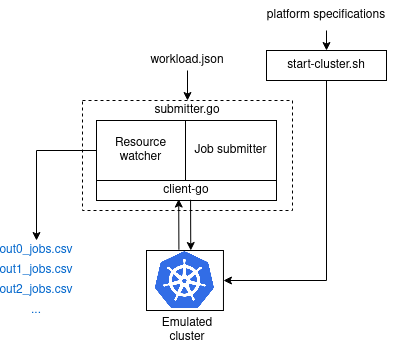
\includegraphics[scale=0.7]{./imgs/prot-k3s.png}
	\caption{An emulated experiment.}
	\label{fig:emulated-expe}
\end{figure}

Figure \ref{fig:emulated-expe} illustrates how this is done. First, we create a
k3s cluster run using docker-compose, which is a tool enabling us to
conveniently create one or several network of containers. Our cluster contains
one master node and several workers which will run our pods. Then, a Go script
which takes a Batsim workload as an input submits the jobs at the right time,
watches the cluster state regularly, and writes the ouputs to csv files --
which have the same format as Batsim's csv output files. We run each workloads
10 times in order to get statistically meaningful results, except for the
realistic workload which we could only run once.

The emulated cluster is limited in terms of variety and capacity. First,
\texttt{start-cluster.sh} only allows the nodes to have the same amount of
available cpu, memory or storage because there was no need for any complex
system for our experiences. Secondly, the maximum amount of cpu, memory or
storage we can make available for each node is capped to the host system
capacities. For example, if the host system possesses 8 cpu cores, the nodes
will have a maximum of 8 cpu available. This will have implications when trying
to run workloads recorded on real systems: either we get to find a workload
that complies with the host system capacity (which is very unlikely), or we
adapt the workload so the jobs requirements do not exceed the host
capabilities (see section \ref{sec:studied-workloads}).

\subsection{Studied workloads} \label{sec:studied-workloads}

We consider three workloads, representing three different situations. The first
two are simplistic and very controlled, and the last one depicts a more
realistic case. In all cases the required resources are only quantified in cpu
only to simplify the study. Note that Batkube does support memory requets, we
just do not wish to add this other layer of complexity to our experiments.

\begin{itemize}
	\item A \textit{burst} workload, consisting in an important amount of
		jobs submitted at once.  200 delays with duration 170s and
		requesting 1 cpu are submitted at the origin.
	\item A \textit{spaced} workload, where jobs of the same nature are
		submitted at regular intervals.  200 delays with duration 170s,
		and requesting 1 cpu are submitted every 10s.
	\item A \textit{realistic} workload, which is a trace extracted from
		the Karlsruhe Institue of Technology ForHLR II System. It is
		composed of 49 jobs including both long running jobs (truncated
		up to an hour) and groups of smaller jobs often submitted
		simultaneously, spanning over 10 hours.
\end{itemize}

The first two workloads are straight forward and could be generated with the
use of a plain text editor (understand \texttt{vim} and its macros). The third
workload required more processing to be obtained.  

\subsubsection{Standard Workload Format processing}

Batsim provides a tool to translate SWF files to its own json definition. It
also works as a workload preprocessor, although we want to process SWF files
very specifically to suit our needs which is why a custom script was
implemented.

First, a trace in standard workload format (swf) was obtained on a web
archive\footnote{\url{https://www.cs.huji.ac.il/labs/parallel/workload/logs.html}}.
The chosen workload was \texttt{KIT-FH2-2016-1.swf} (we give the file name for
the reader to find the workload on the archives) because it is the most recent
and is relatively lightweight. It is composed of 114,355 jobs spanning over 19
months. Secondly, \texttt{evalys}\footnote{\url{https://github.com/oar-team/evalys}}
allowed us to extract a subset of this workload lasting for a given period of
time and with a given mean utilization of the resources. We chose a period of
10h with 80\% utilization of the resources so as to keep reasonable experiment
durations -- Later on we experiment with larger workloads to test out Batkube's
limits in terms of scalability.  The third step is translating this extracted
workload to a \texttt{json} file that can be read by Batsim.

After extracting this subset, we are left off with a workload containing jobs
spanning up to 45h and using up to 24048 cpu (or cpu cores), which is undoable
at our scale on our emulated cluster. We need to trim job durations as well as
cpu usage, as we are limited in cpu by the host machine. This is done during
the translation to the \texttt{json} format. The durations are trimmed down to
a maximum of one hour and the cpu usages are normalized so the maximum amount
of cpu requested equals the amount of cpu available per node on the host
machine. Otherwise, the job would not be schedulable which would not present
much interest. We end up with a trace composed of 39 jobs spanning over 10
hours, with a maximum job length of one hour and cpu usage ranging from 0
(excluded) to 5.9 (even though the host machine had 6 cores, Kubernetes
scheduler did not allow for a job to be scheduled on a node it would use 100\%
resources of).

\subsection{Studied platforms}

The platform used for the first two workloads, \textit{burst} and
\textit{spaced} is composed of 16 nodes each heaving one cpu. For the
\textit{realistic} workload however, we use a single node composed of six cores
for the following reasons.

First, the host machines where the experiments were conducted had six cpu cores
available. This means that if we want to be able to run an emulated cluster
equivalent to this platform we can't exceed six cpu per node.  We use the
maximum amount of available cores to avoid obtaining too low values
when normalizing the resource requests on the jobs. Indeed, Kubernetes only
allows for a precision of 1 milicpu, so any value bellow that is not considered
a significant number. Normalizing on six cpus instead of one allows us to get
more significant number. Also, only one node gives us a satisfactory overall
resource usage: with more than one node one resource is almost always available
making the scheduling operations trivial.


\section{Study of the simulator parameters} \label{sec:params-eval}

The simulator has a few parameters that impact the simulation speed and
accuracy. The objective is to study the effects of these parameters on the
simulation to better understand the scheduler behavior when running in
coordination with Batkube.\\

The objective here is to fine tune the parameters in order to find a compromise
between accuracy and scalability. We want to know which combination lead us to
the most stable results, while keeping simulation time as low as possible. In
these simulations, the scheduling time is very low and was neglected.  This
would not be the case with more complicated workloads involving complex
scheduling mechanisms.

The parameters are:
\begin{itemize}
	\item The \textit{minimum delay} we have to spend waiting for the
		scheduler.
	\item The \textit{timeout} value when waiting for scheduler decisions.
	\item The \textit{maximum simulation time step}, which is the maximum
		amount of time Batsim is allowed to jump forward in time.
\end{itemize}

We first study these parameters one by one by fixing the other parameters, then we study what effects these parameters have in respect
to one another. Finally we conduct scalability experiments to test
Batkube's stability and performances on large workloads.

\subsection{Minimum delay}

Earlier in the development of batkube we noticed that not leaving enough time
to the scheduler each cycle lead it to crashes and deadlocks, ultimately
failing the simulation. This time is independent from any decision making we
would receive from it. Which is why it is called \textit{minimum wait delay}
instead of a plain \textit{timeout} - which is in fact another parameter we
will study later.

For each workload, we compute the crash rate every 5ms, from 0ms to 50ms. Each
point is made by running the simulation 15 times and recording the exit code as
well as the simulation time. The other parameters are: \texttt{timeout=20ms};
\texttt{max-simulation-timestep=20s}. As we will see later those do not offer
acceptable simulation results but they allow us to run prompt simulations, as
accuracy do not concern us here.\\

\begin{figure}
	\centering
	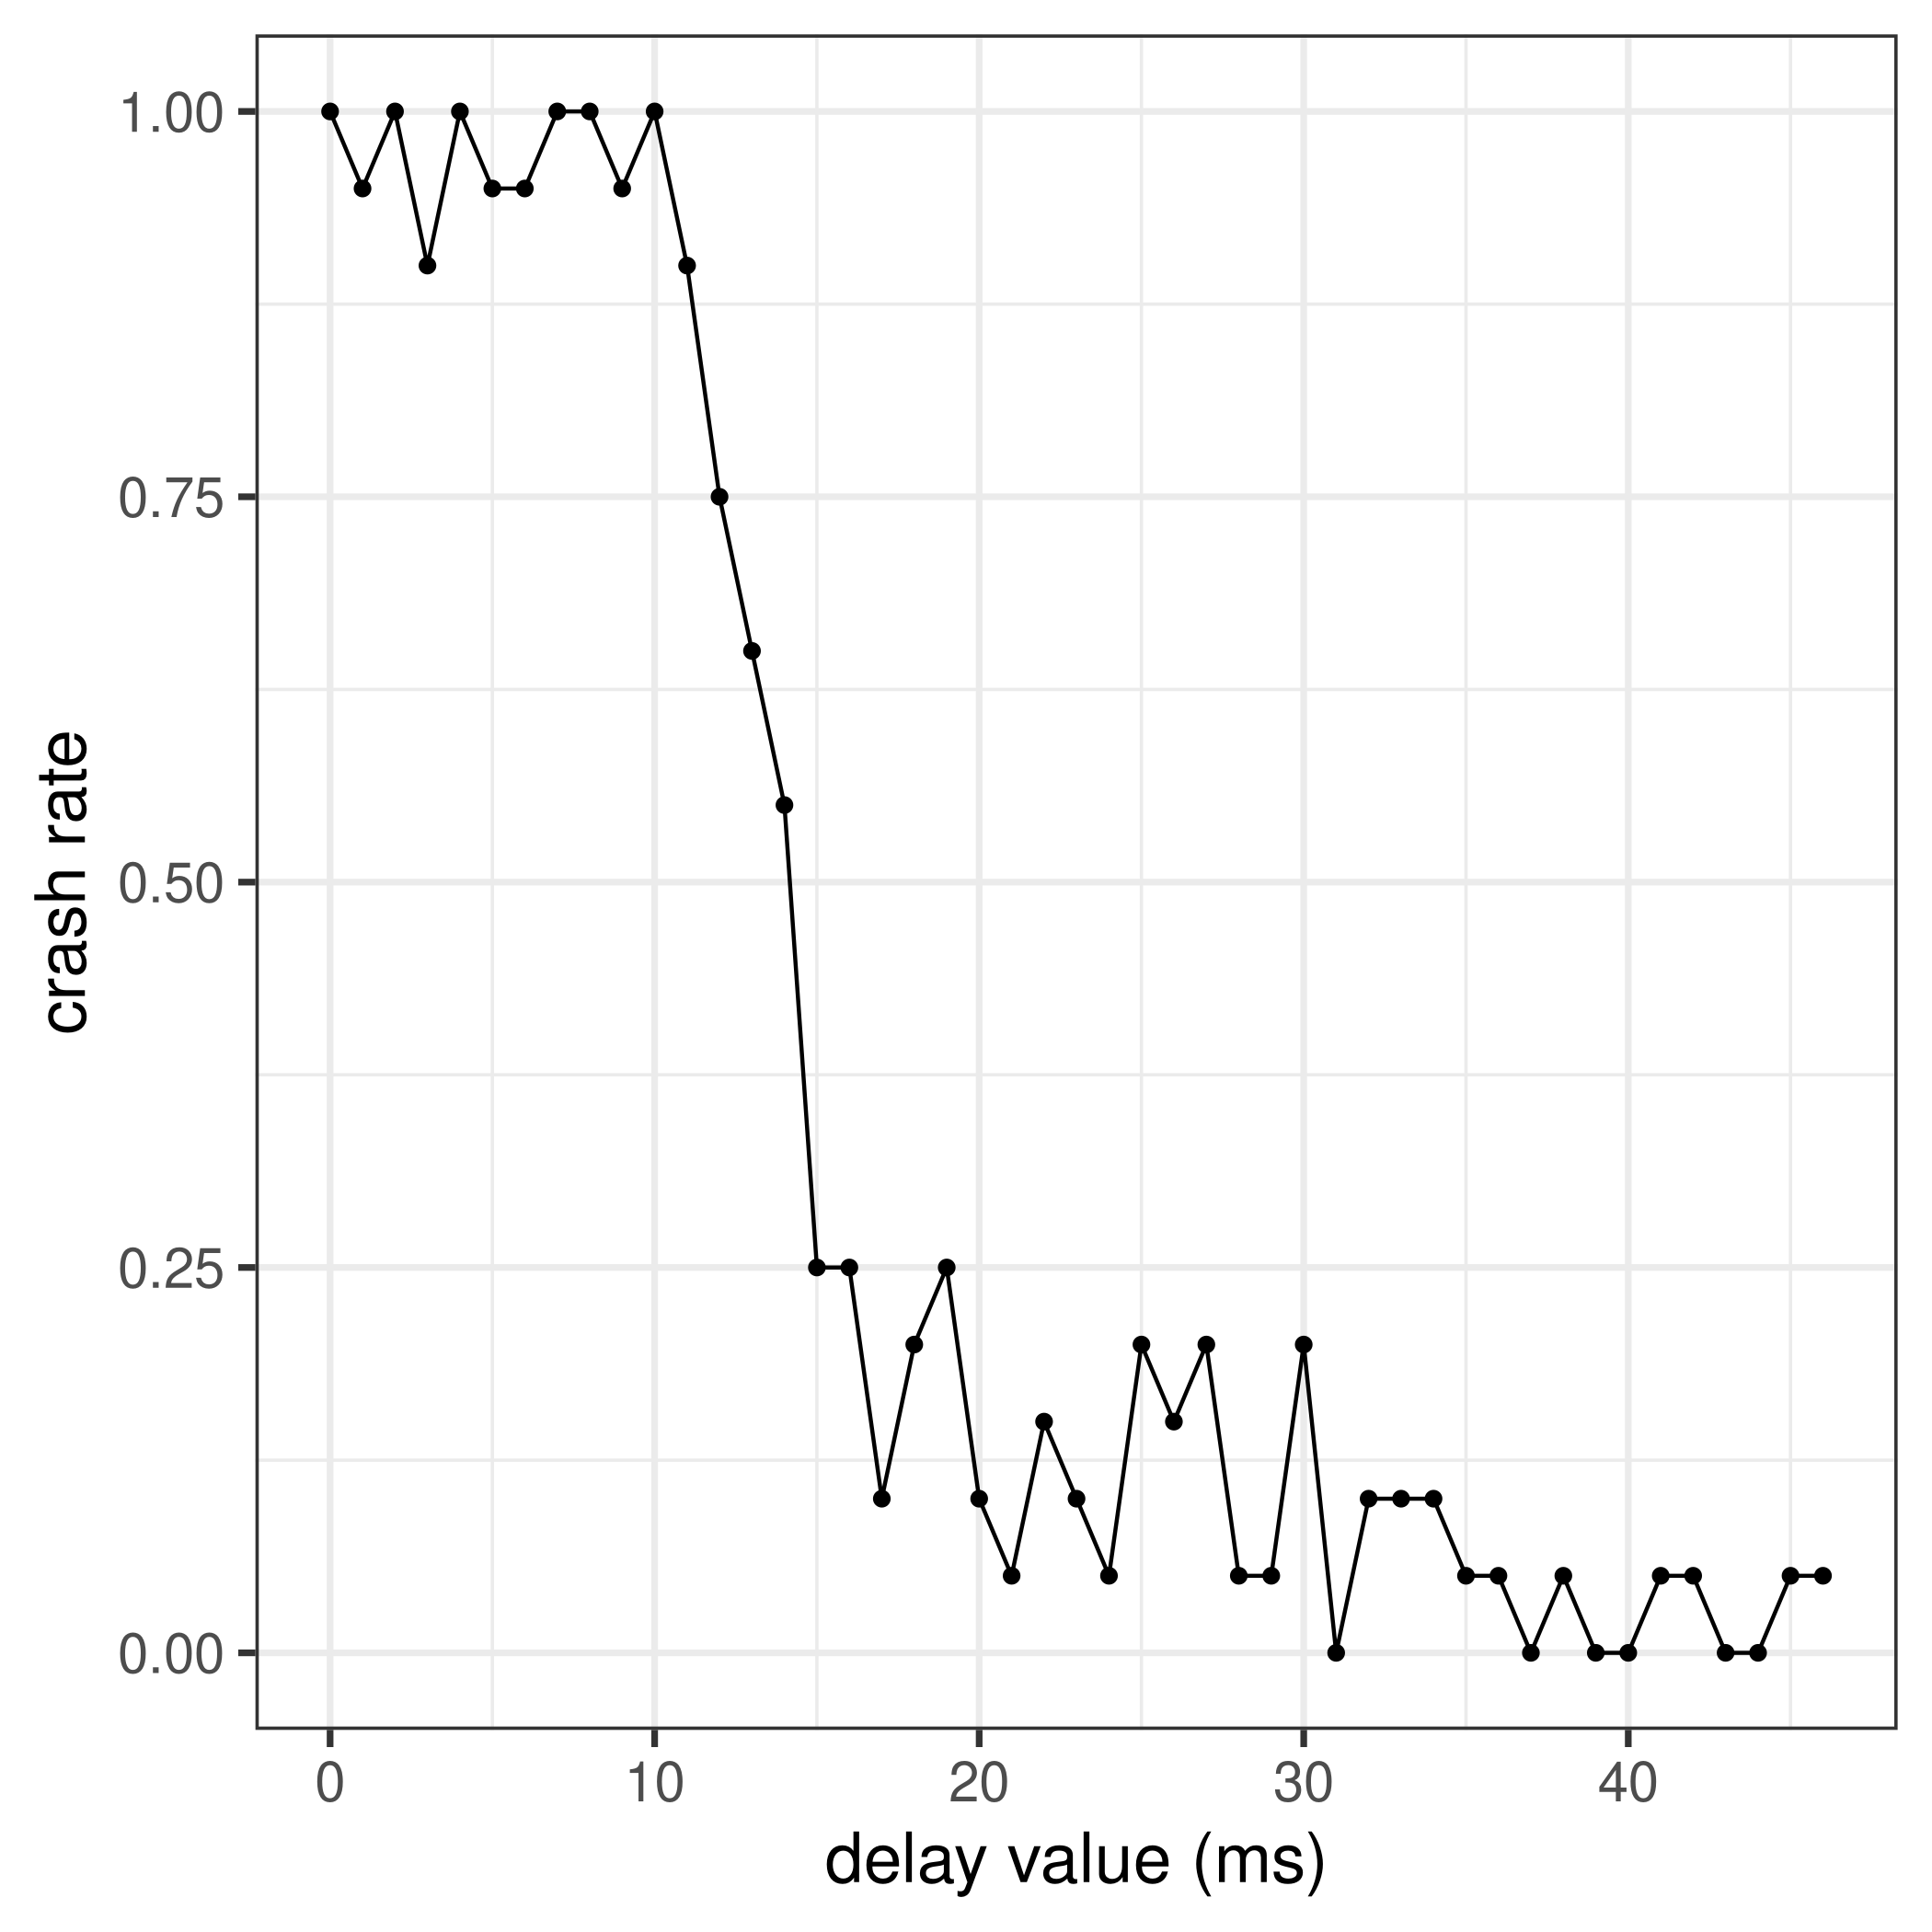
\includegraphics[width=0.5\textwidth]{imgs/min-delay_crash_old.png}
	\caption{Crash rate of the simulations against minimum delay.}
	\label{fig:min-delay_crash}
\end{figure}

\begin{figure}
	\centering
	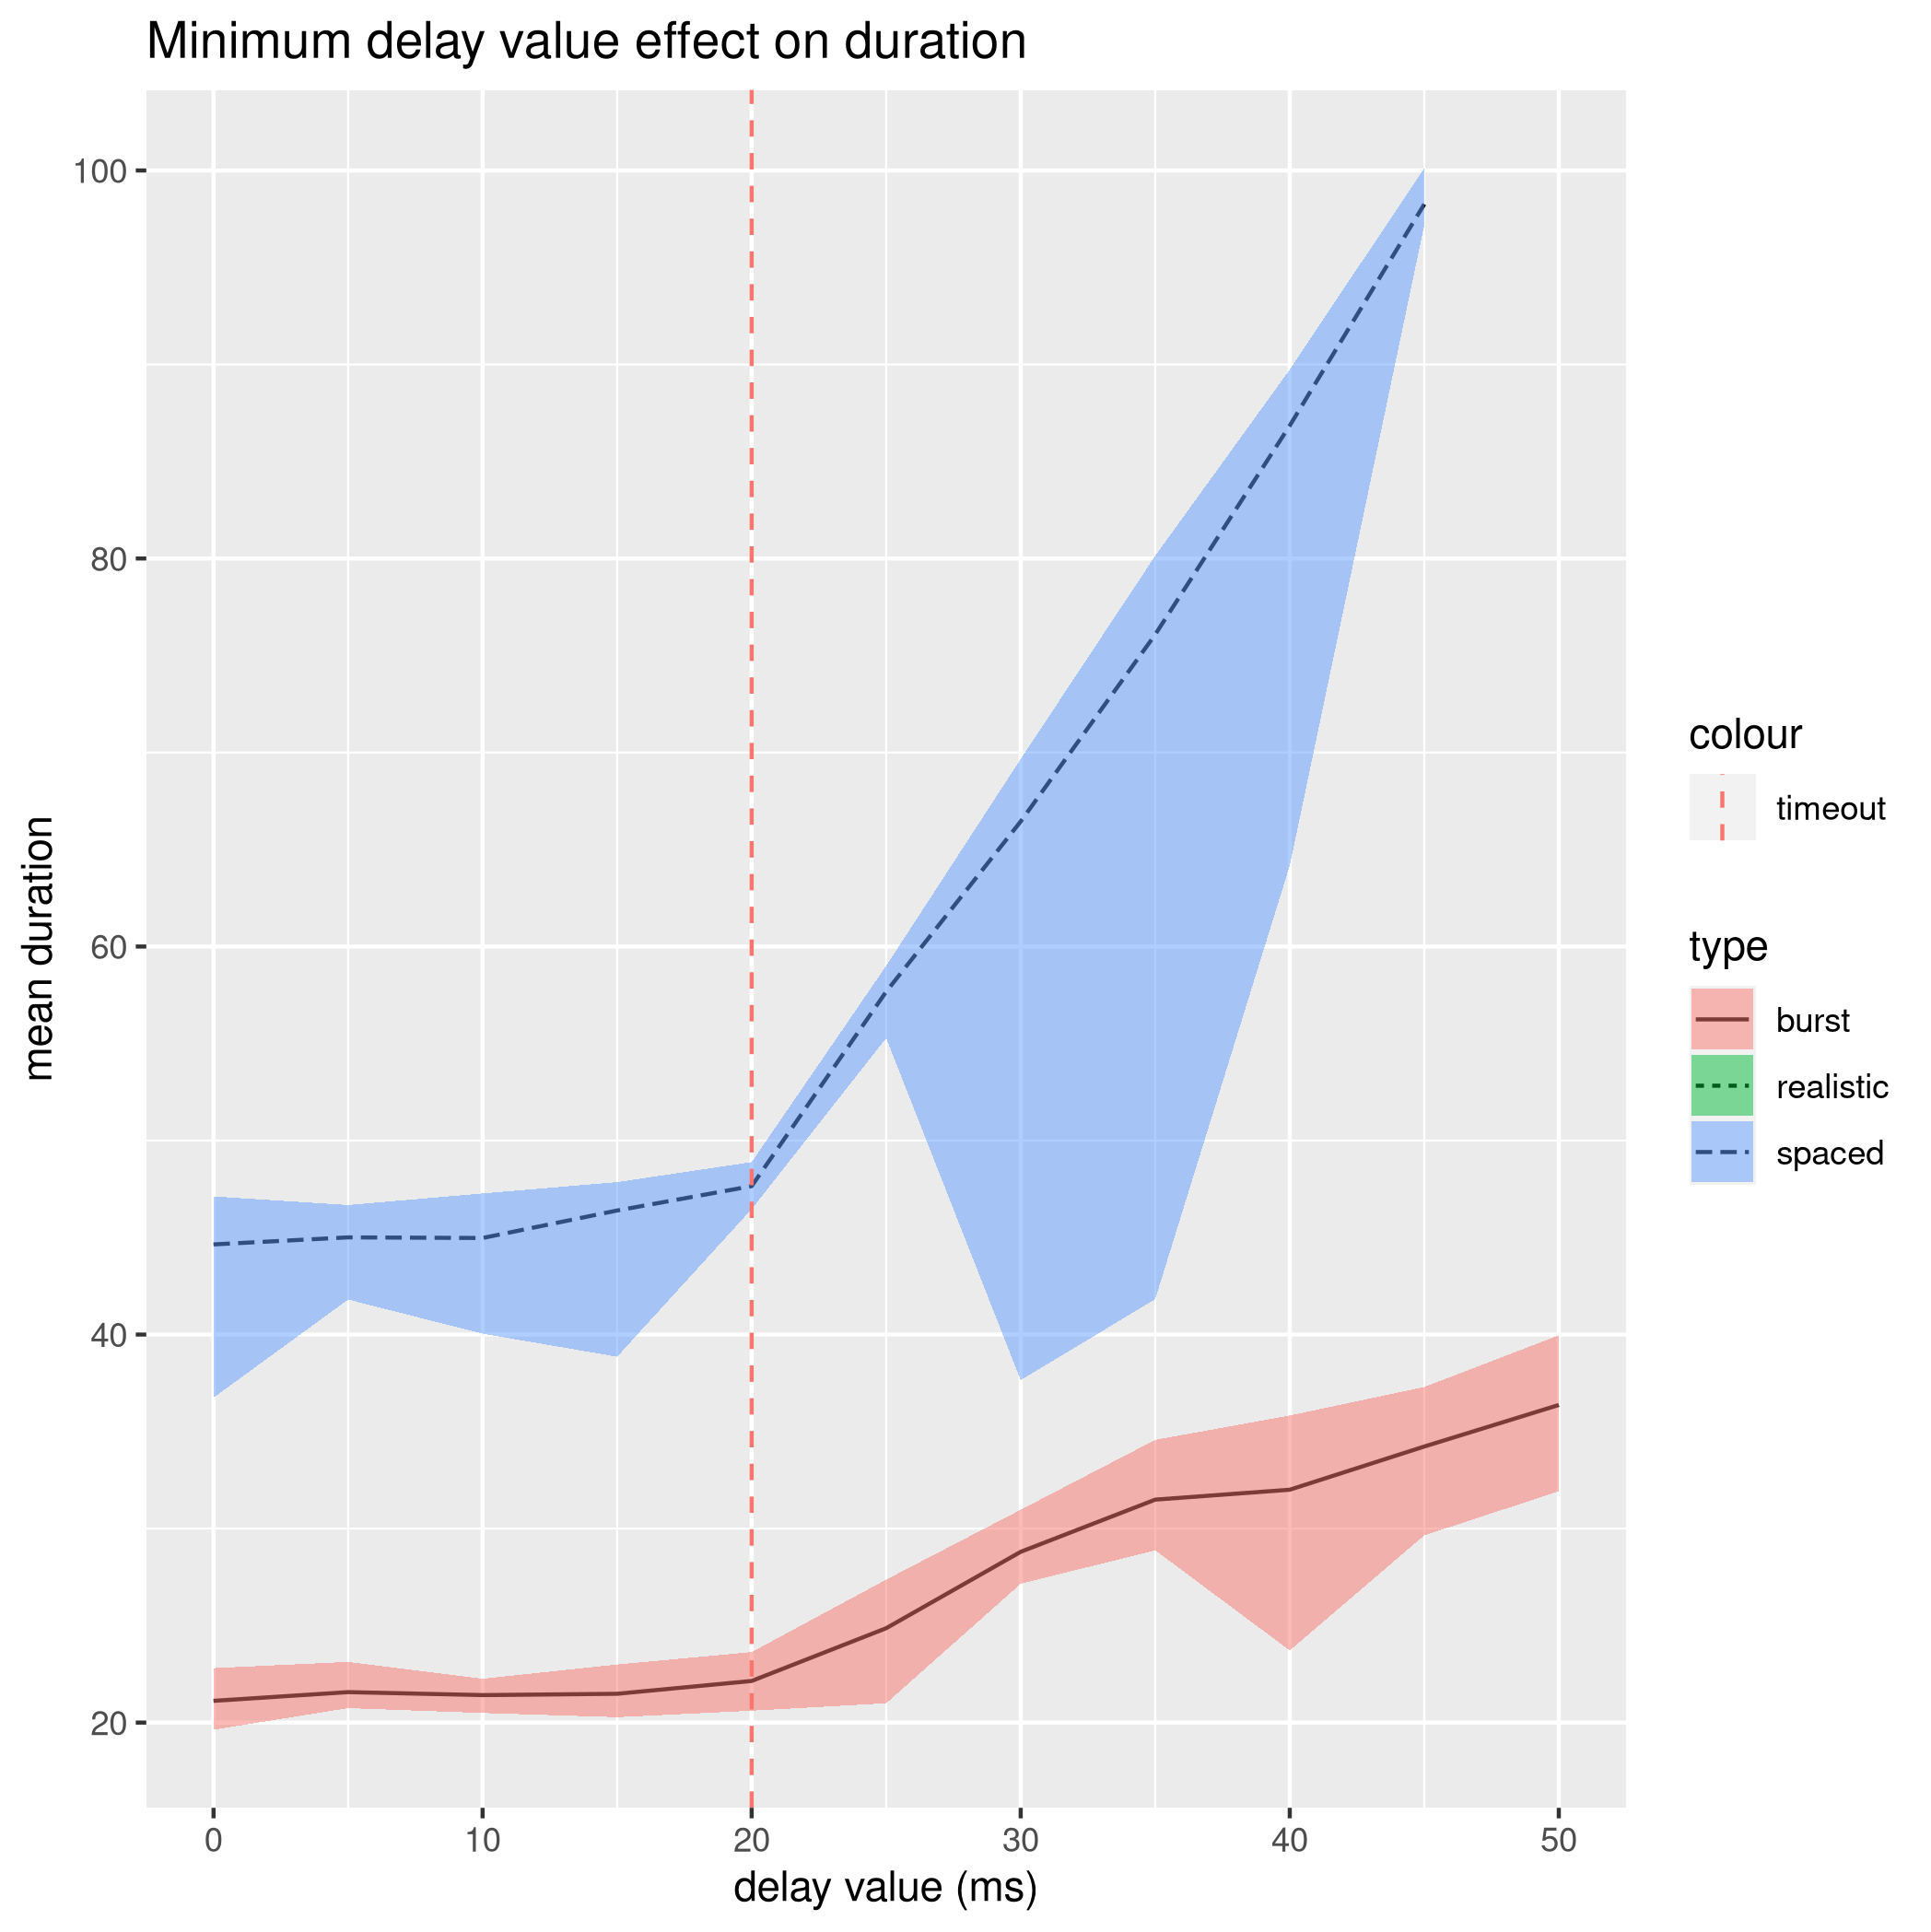
\includegraphics[width=0.9\textwidth]{imgs/min-delay_duration.png}
	\caption{Mean duration of the simulations (in case of success) against minimum delay. Error bars show confidence intervals at 95\%.}
	\label{fig:min-delay_duration}
\end{figure}

As we can see on figure \ref{fig:min-delay_crash}, the crash rate decreases
dramatically as soon as the minimum delay reaches a certain threshold, which
here is 10ms.  This crashing issue though was resolved with an update of the
scheduler : the success rate flattens out at 100\% -- or around 100\%. Then,
with earlier versions of the scheduler, the user may have to adjust the minimum
delay in order to run simulation smoothly. 

We also observe on figure \ref{fig:min-delay_duration} -- which was made with
an updated scheduler -- a prompt increase in simulation time from delay value
20ms. This is due to the fact that the \textit{timeout} value is 20ms, which is
reached most of the time because the vast majority of the calls to the
scheduler do not result in a decision making. After this value, we notice a
direct correlation between \textit{minimum delay} increase and simulation time
increase. It follows that the best choice for the \textit{minimum delay} now is
zero, and we will use this value for the rest of the experiments.

\subsection{Timeout}

This value is the maximum amount of time we leave for the scheduler to react. A
\texttt{timeout value} not large enough may lead to inaccuracies in the
simulation: for example, if the scheduler needs 30ms to make a decision upon
reception of a message, and the value of the timeout is 20ms, Batkube will
receive the decision on the next cycle which may happen several dozens of
seconds later (depending on the \textit{maximum simulation time step} value).
This phenomenon appears very clearly in figure \ref{fig:timeout_gaps} which
represents a simulation run on the spaced workload (other parameters are
\texttt{min-delay=0} and \texttt{max-simulation-timestep=1000s} to reduce
simulation time). Additionally, this graph shows us that low timeout values
induce incorrect behavior from the scheduler such as over allocation of
resources: darker areas show jobs overlapping on the same resource, even though
all resource have a capacity of one cpu and jobs request one full cpu.  On the
other hand, a \textit{timeout value} too large will induce longer simulation
times. Indeed, once the simulator was given enough time to process a message,
any time following is spent idling. We want to measure which \texttt{timeout
value} is just enough for the scheduler to be able to make a response without
spending any time idling.

We run each workload with a \texttt{timeout value} ranging from 0ms to 100ms,
--except for the realistic workload because simulation times were already
consequent from 50ms -- with a step of 1ms. Each time we measure the duration
of the simulation as well as the makespan and the mean waiting time. The latter
two will enable us to compare the results against the emulated results in order
to estimate the accuracy of the simulation. The other parameters are set to:
\texttt{min-delay=0ms}, \texttt{max-simulation-timestep=20s}

\begin{figure}
	\begin{subfigure}{0.5\textwidth}
		\centering
		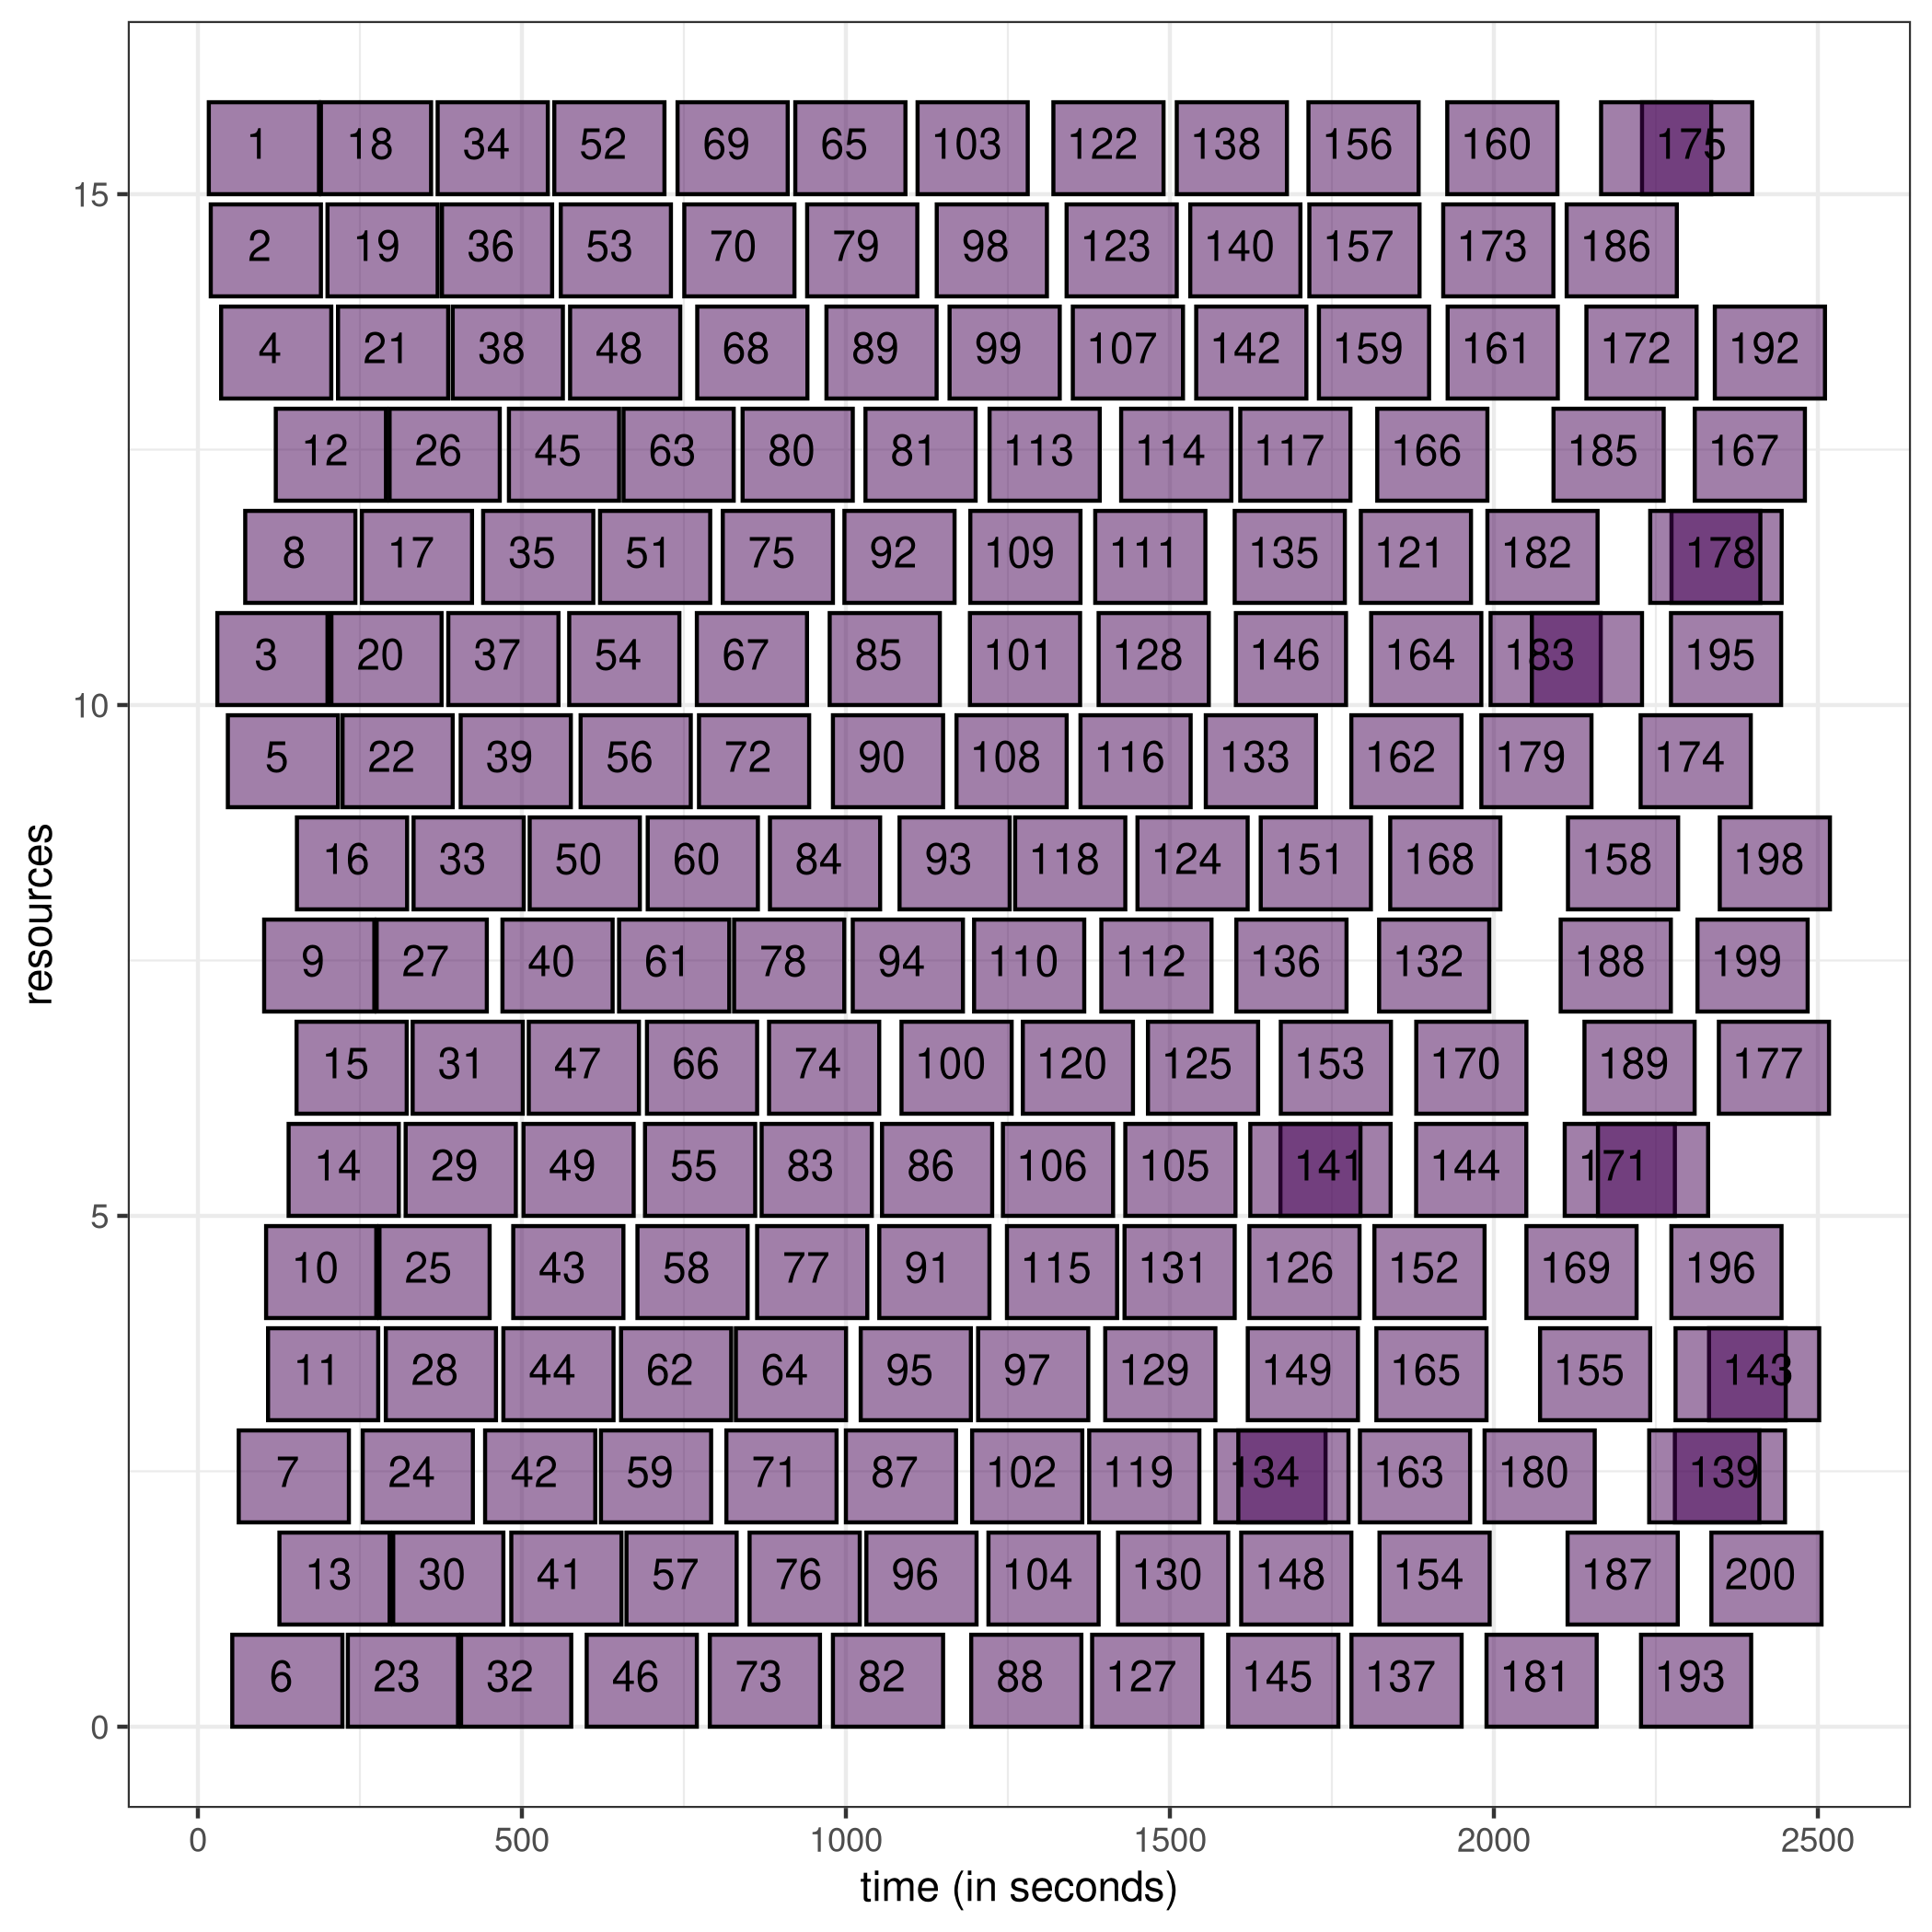
\includegraphics[width=\textwidth]{imgs/timeout_5ms_gantt.png}
		\caption{Timeout value: 5ms}
		\label{fig:timeout_5ms}
	\end{subfigure}
	\begin{subfigure}{0.5\textwidth}
		\centering
		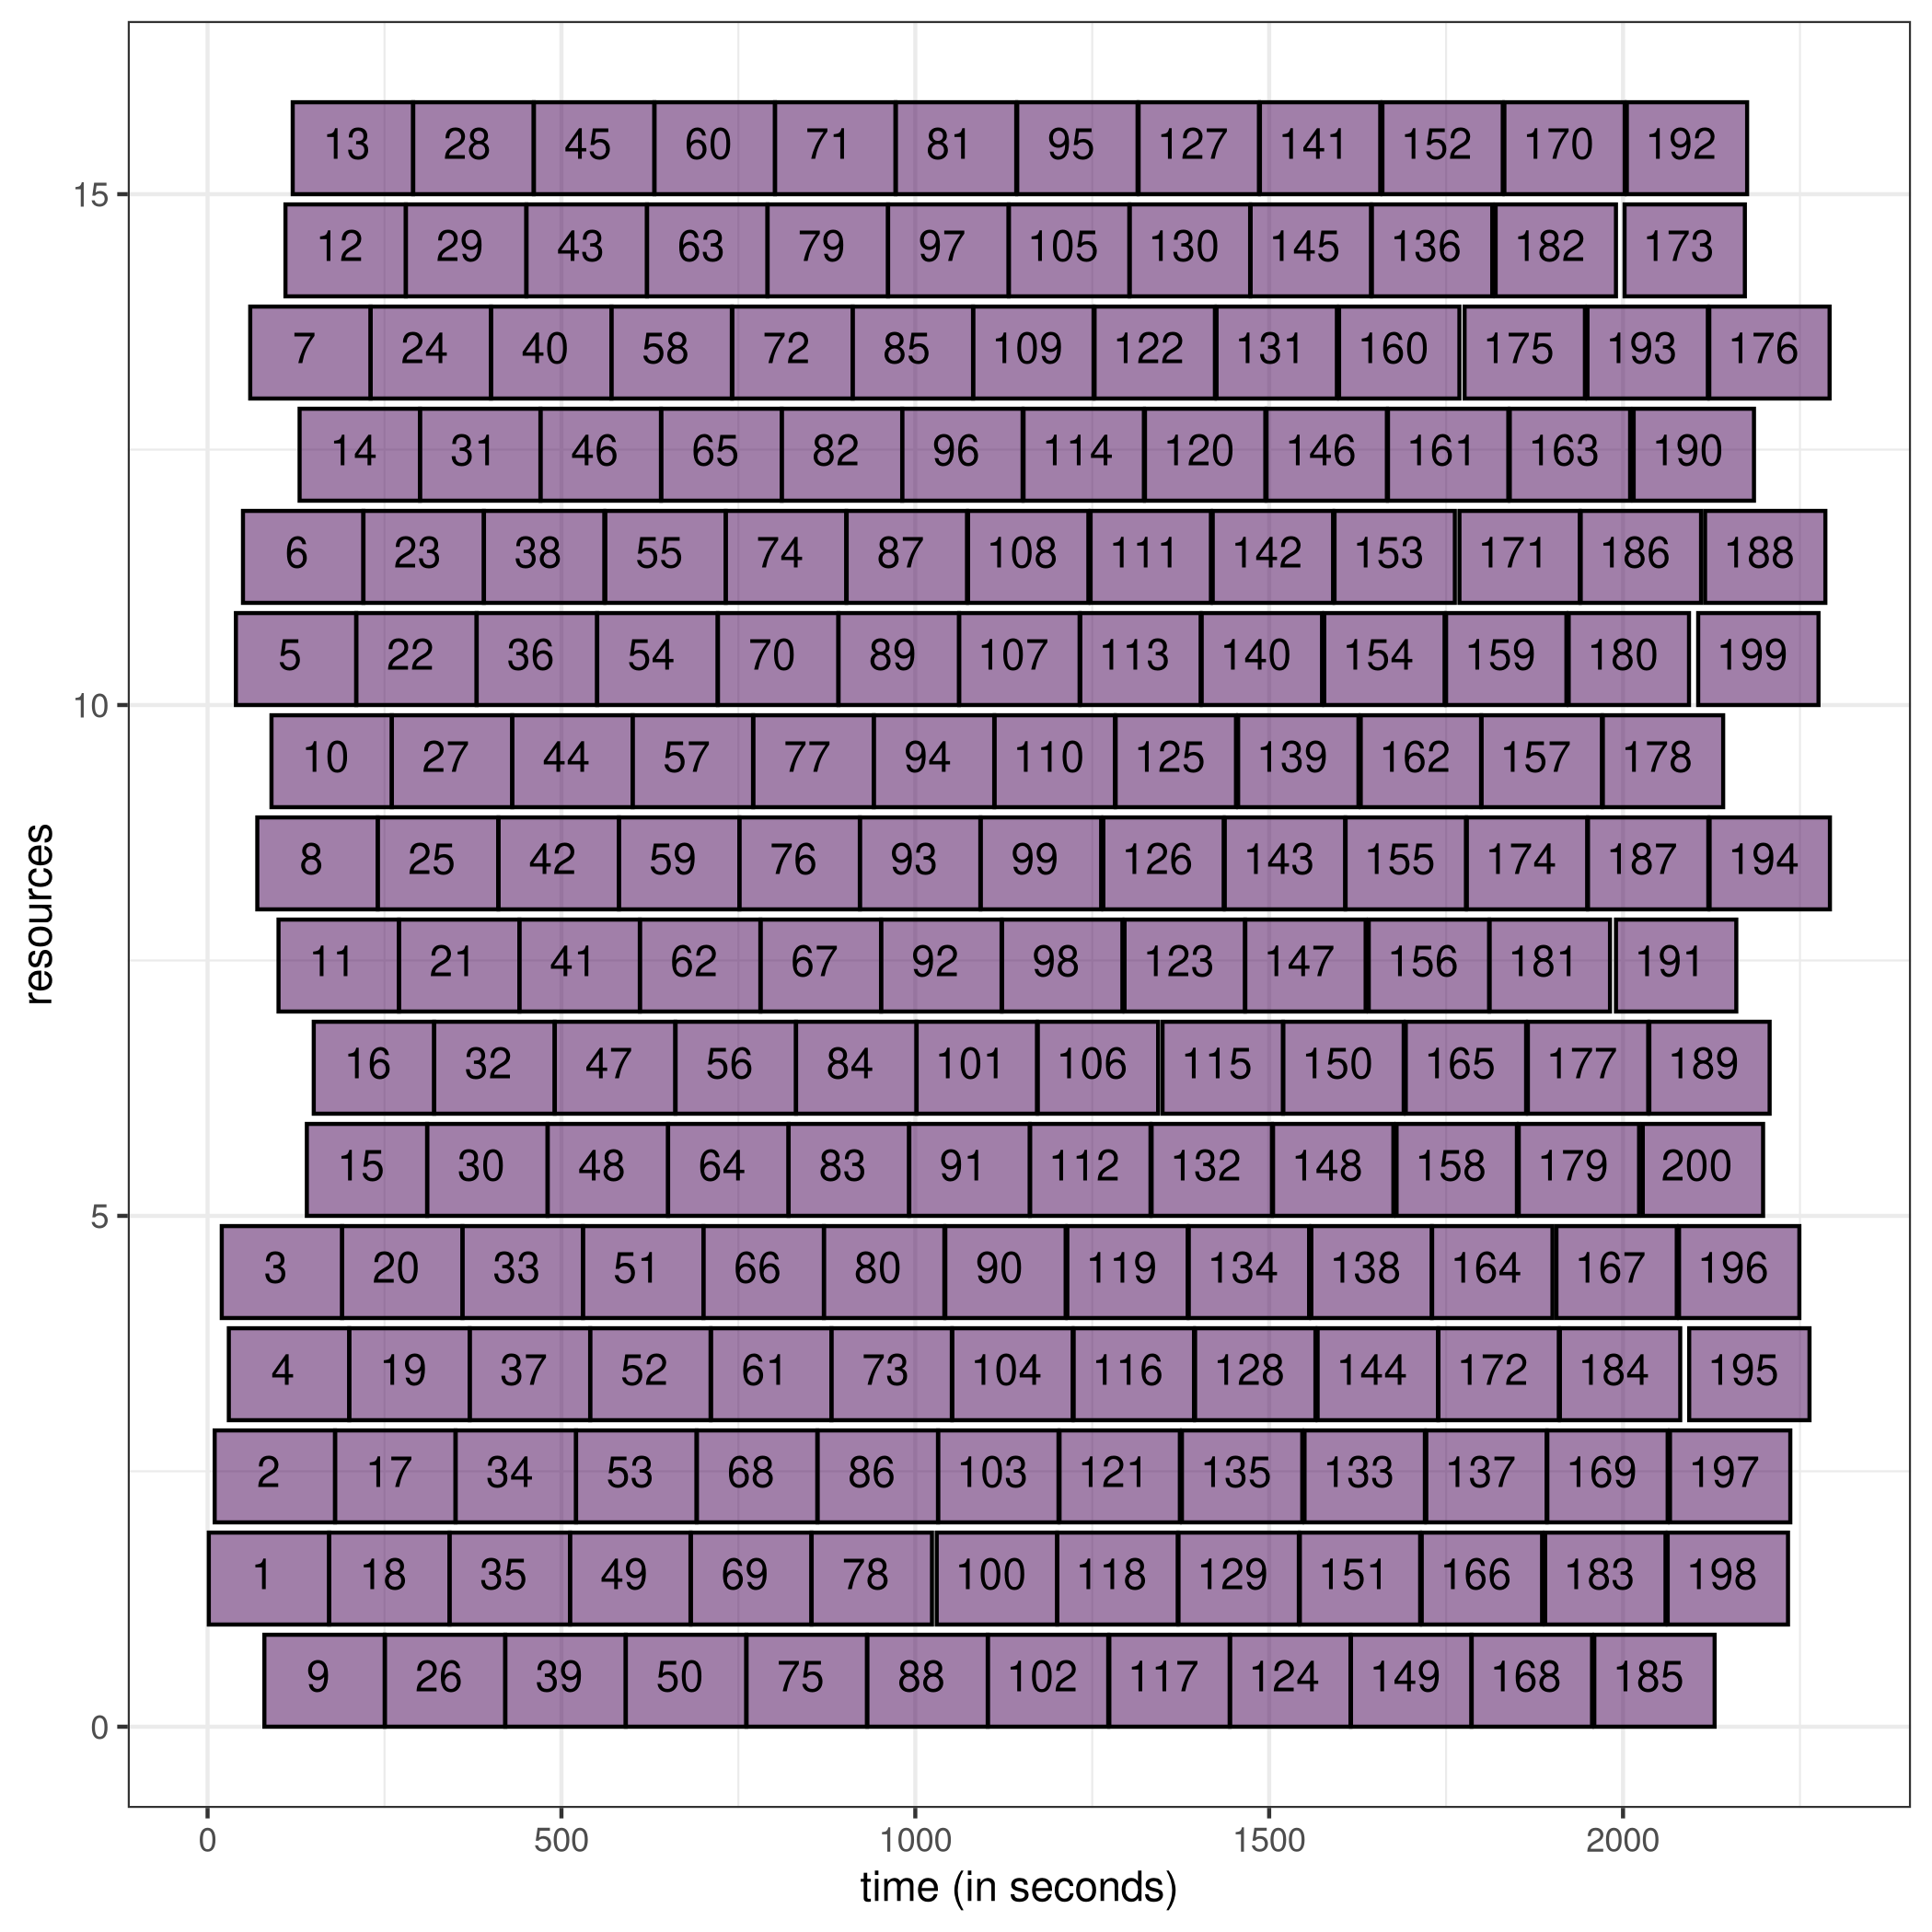
\includegraphics[width=\textwidth]{imgs/timeout_50ms_gantt.png}
		\caption{Timeout value: 50ms}
		\label{fig:timeout_50ms}
	\end{subfigure}
	\caption{A low timeout value results in the apparition of delays in the scheduling process. Both gantt charts were made with the \textit{spaced} workload.}
	\label{fig:timeout_gaps}
\end{figure}

\begin{figure}
	\begin{subfigure}{\textwidth}
		\centering
		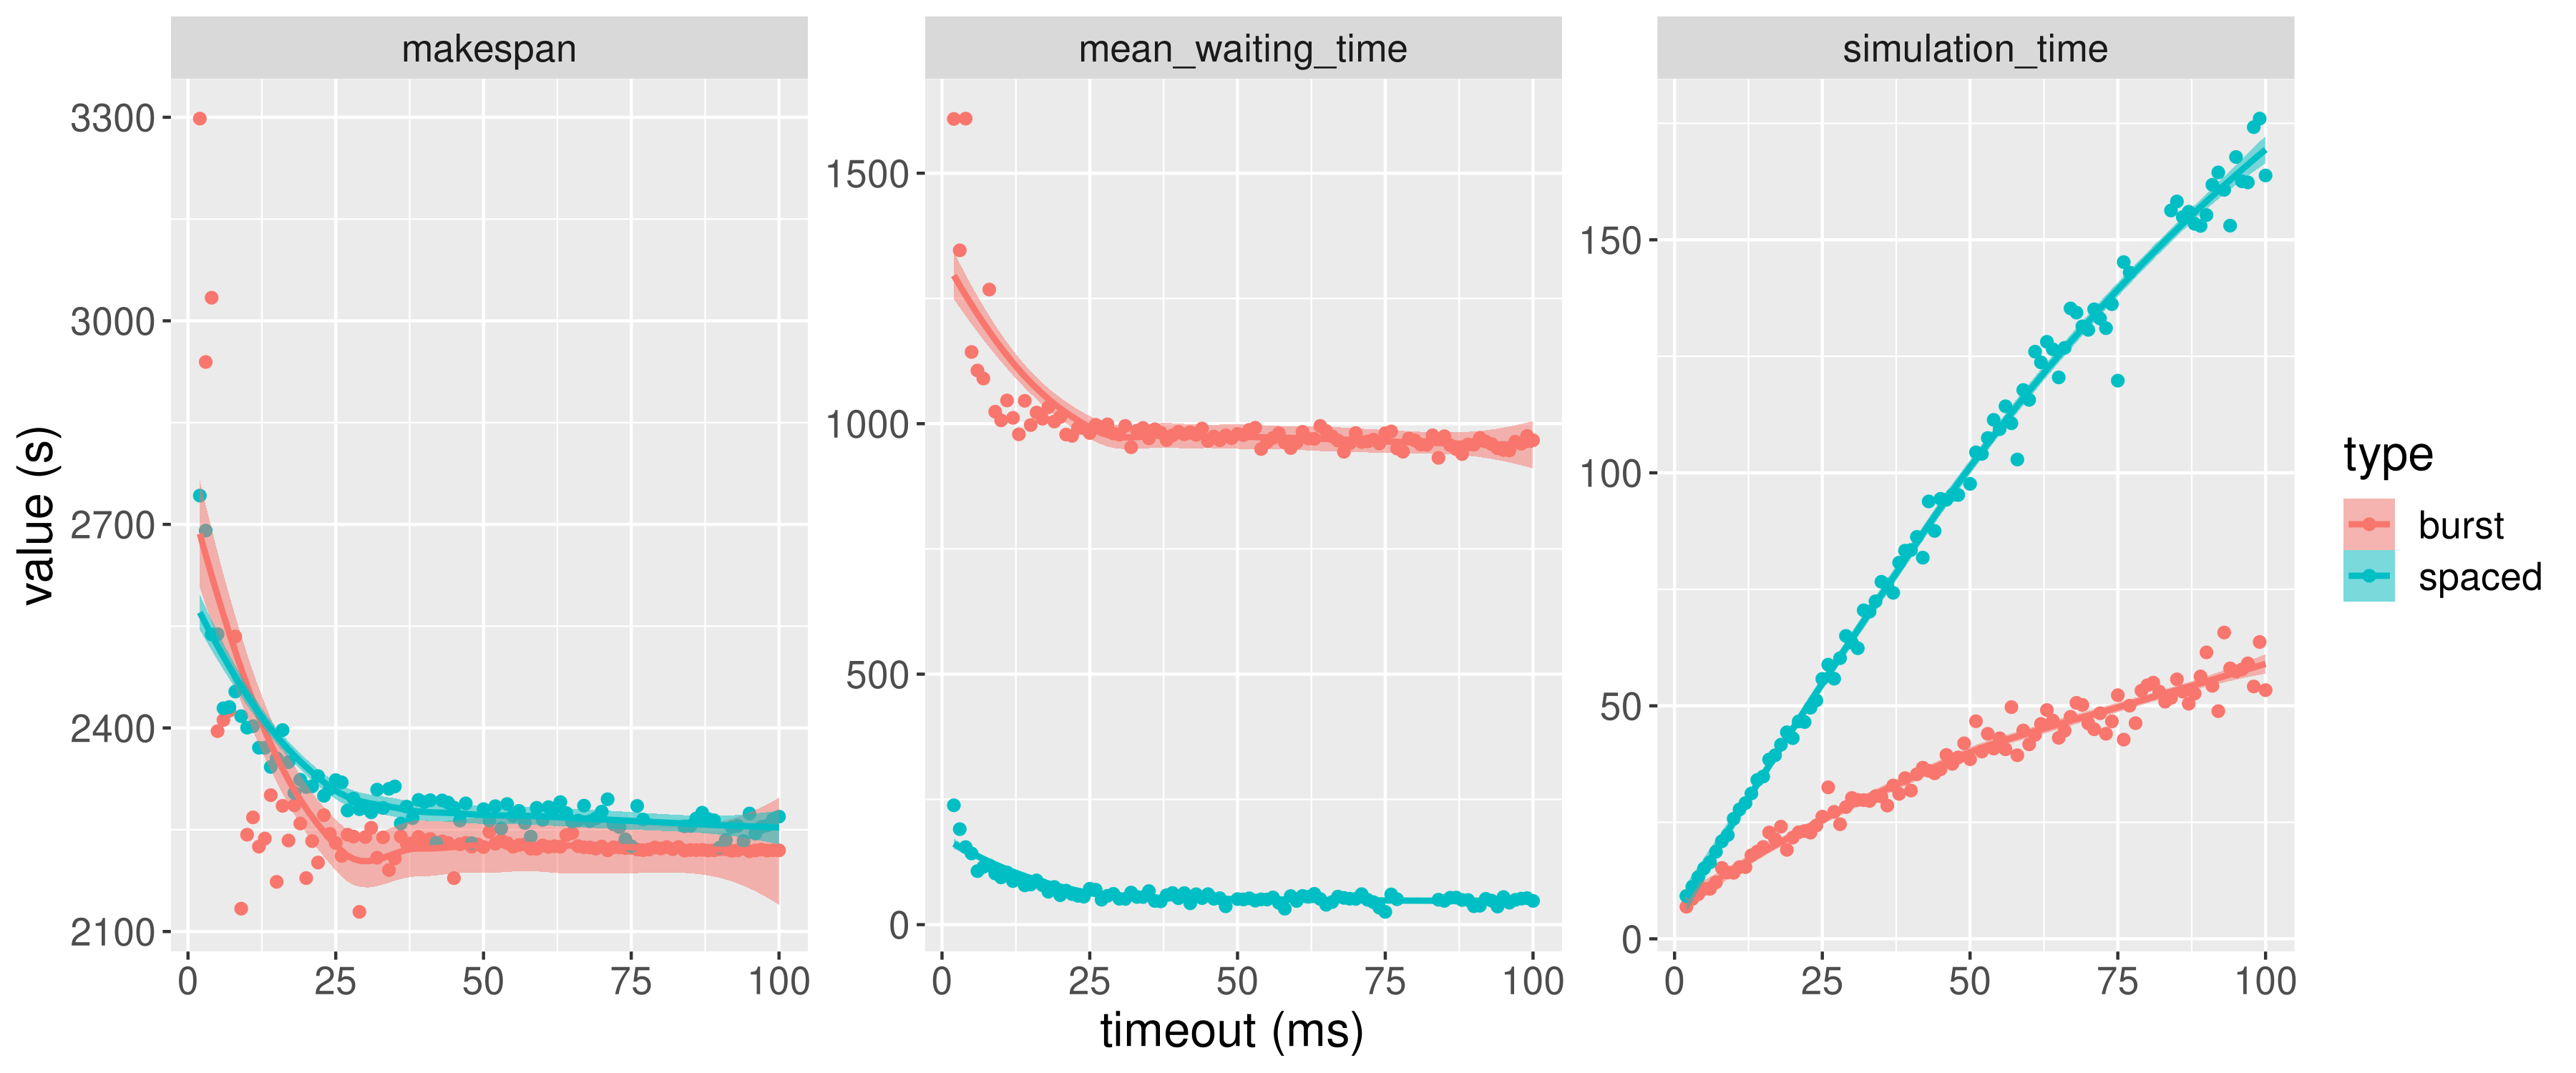
\includegraphics[width=\textwidth]{imgs/timeout_burst_spaced.png}
		\caption{}
		\label{fig:timeout_burst_sp}
	\end{subfigure}

	\begin{subfigure}{\textwidth}
		\centering
		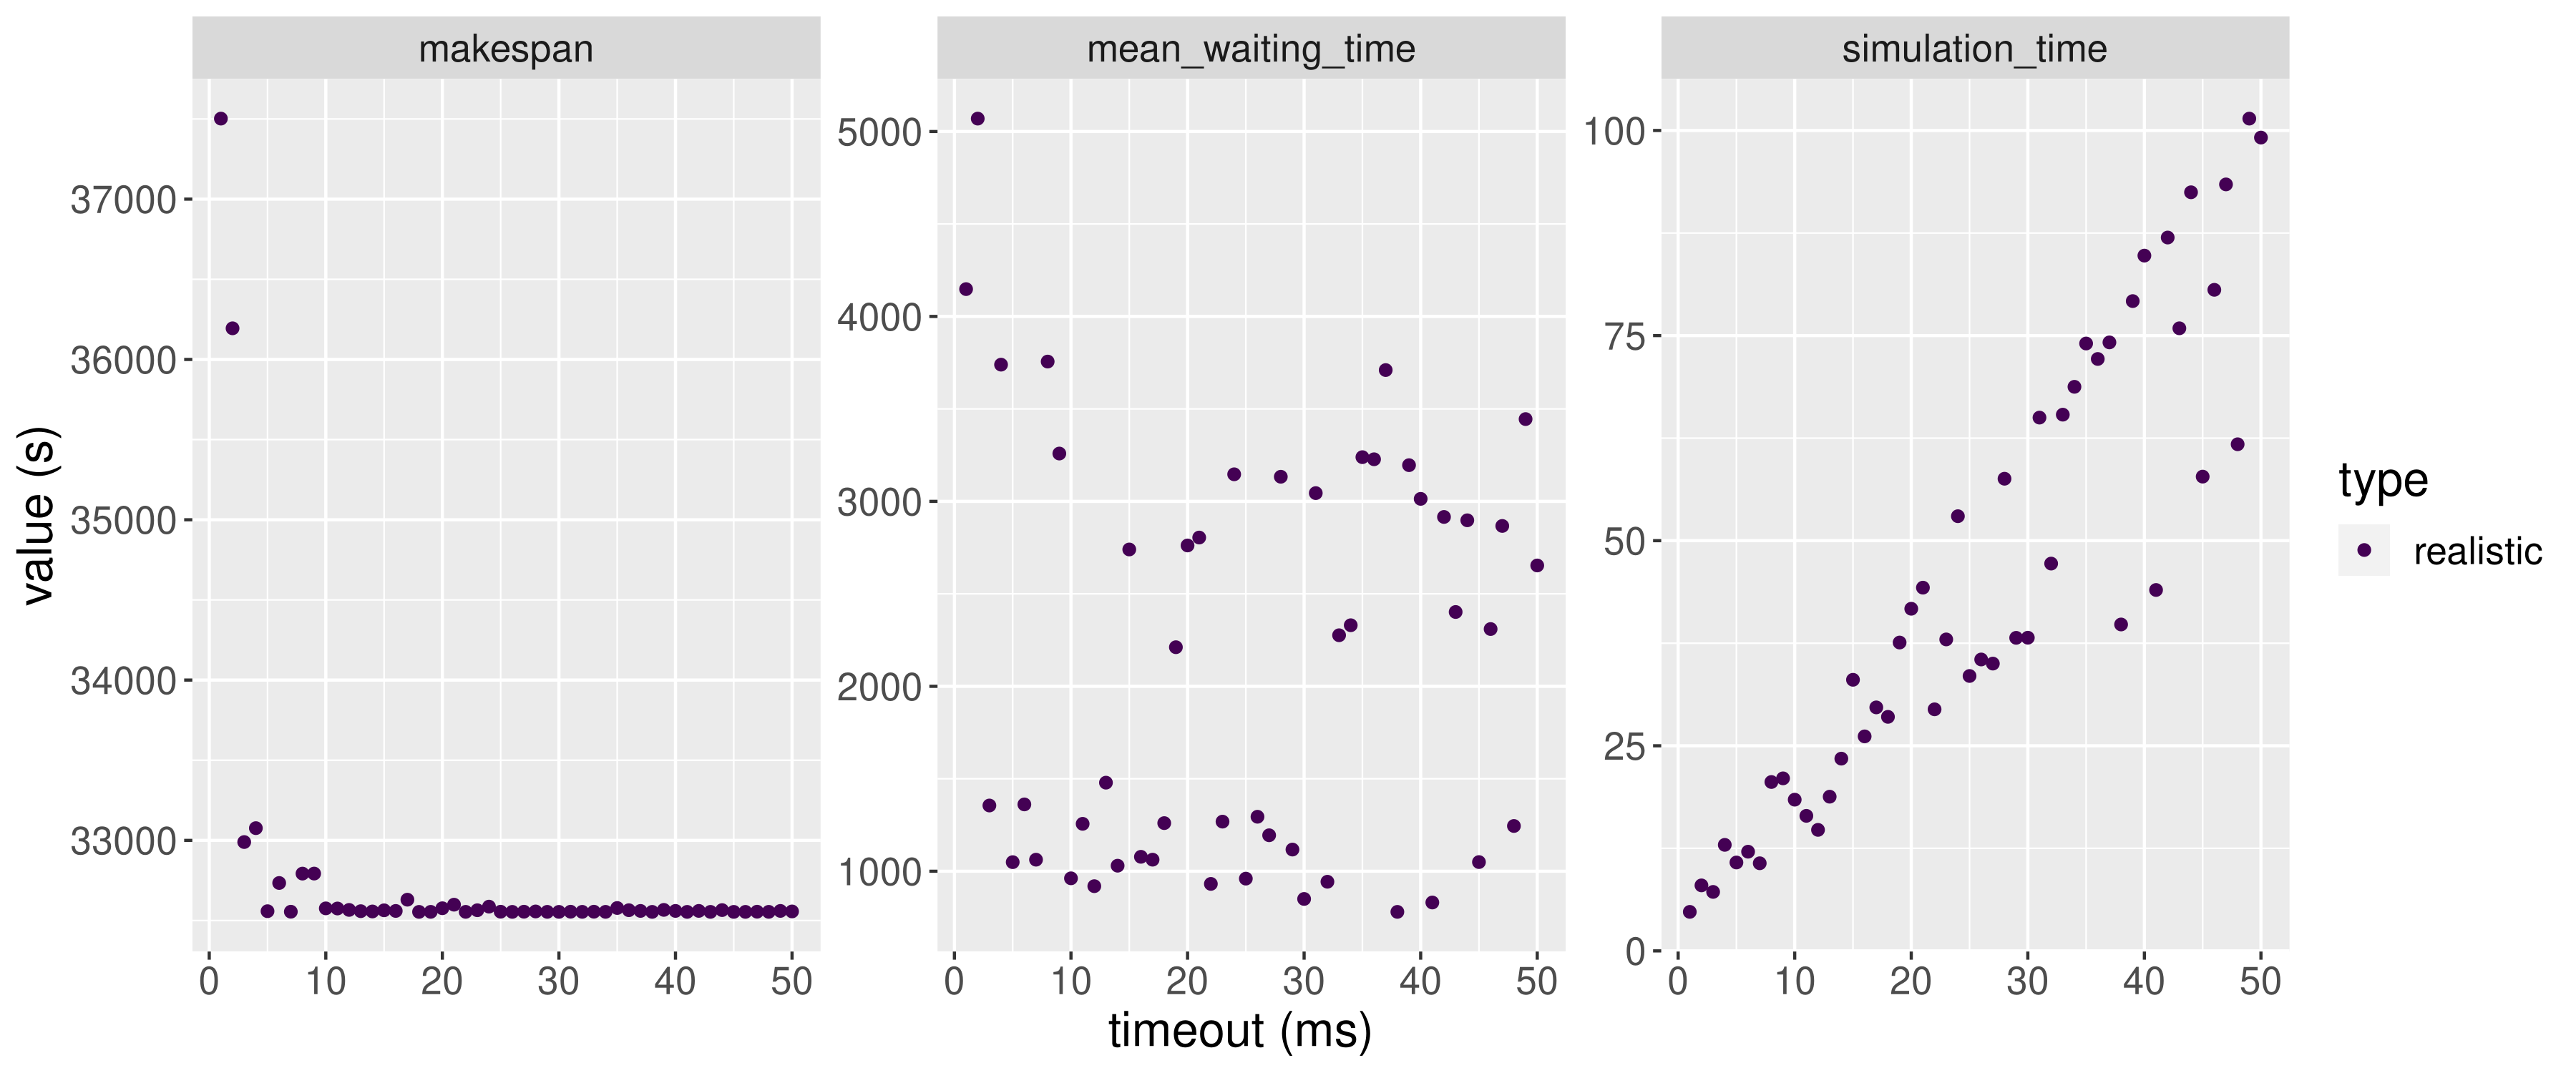
\includegraphics[width=\textwidth]{imgs/timeout_realistic.png}
		\caption{}
		\label{fig:timeout_real}
	\end{subfigure}

	\caption{Effect of the timeout value on the simulation.}
	\label{fig:timeout}
\end{figure}

Figure \ref{fig:timeout} shows the results we obtained. As we expected, a
\textit{timeout value} too low results in the scheduler missing a few cycles
each time it wants to communicate a decision making, thus increasing the
makespan and mean waiting time. As the \textit{timeout} increases, it reaches a
point where the scheduler consistently sends decisions in the same cycle as the
one where it has received the message that triggered the decision making. After
this point though the curves keep decreasing slightly, showing that the gaps
keep receding afterwards. However, the gain in accuracy is shallow and
considering that there is, again, a direct correlation between the
\textit{timeout value} and the simulation time, it is desirable to keep this
value at the limit where the results start to stabilize.  In this case,
according to figure \ref{fig:timeout}, \texttt{timeout-value=50ms} seems a
decent compromise between accuracy and scalability.

We observe slightly different behaviors with the realistic workload. First, the
results stabilize earlier than the other workloads as we can see on the first
graph of figure \ref{fig:timeout_real}. Also, the mean waiting time and
simulation time values are much more scattered than the other two workloads: it
seems like two curves appear on the last two graphs. Since the simulation is
not deterministic, and that the number of jobs in the realistic workload is
fairly low, a slight difference in scheduling decisions has a notable impact on
the simulation. 

\subsection{Maximum simulation time step}

Having a high maximum time step value will allow Batsim to jump forward further
in time. This may result in skipping scheduler decisions that could have been
made in the mean time, delaying them to when Batsim decides to wake up. We
expect increasing this value to have an analogous effect to the timeout value:
higher simulation speed, but also decreased accuracy due to gaps (delays) in
the decision process.

To experiment with the maximum time step effect on the results we obtain, we
run each workload with different values of \texttt{max-simulation-timestep}
following a logarithmic scale. The other parameters are fixed to
\texttt{min-delay=0s}, \texttt{timeout=50ms}. Also, the
\texttt{base-simulation-timestep} was lowered to 10ms in order to test lower
values of the maximum timestep (compared to the previous 100ms).

\begin{figure}
	\begin{subfigure}{\textwidth}
		\centering
		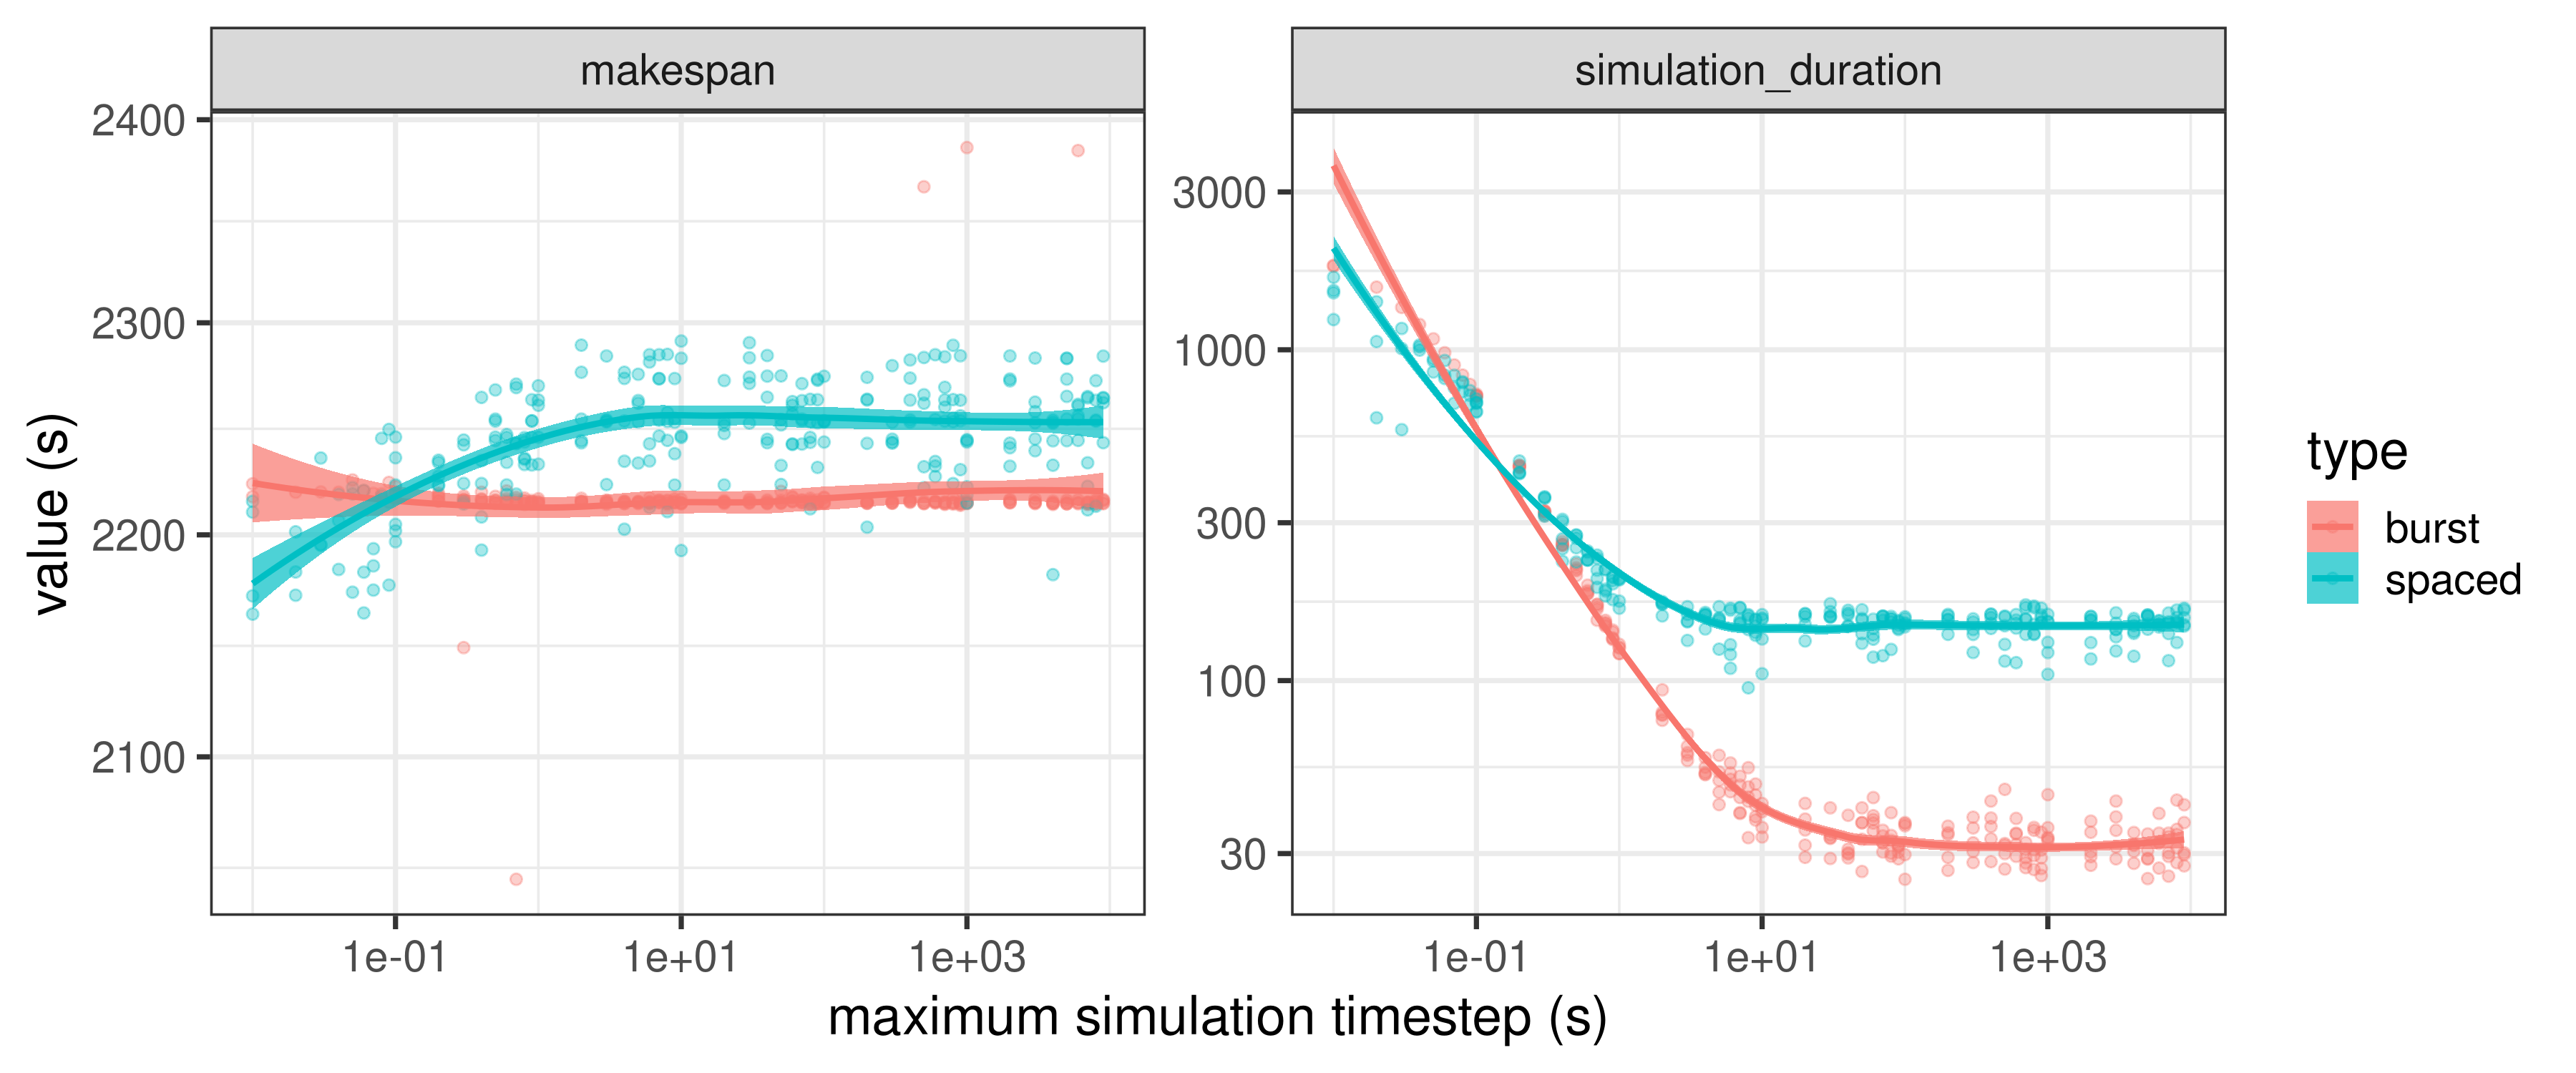
\includegraphics[width=\textwidth]{imgs/max-timestep_burst_sp.png}
		\caption{}
		\label{fig:timestep_burst_sp}
	\end{subfigure}

	\begin{subfigure}{\textwidth}
		\centering
		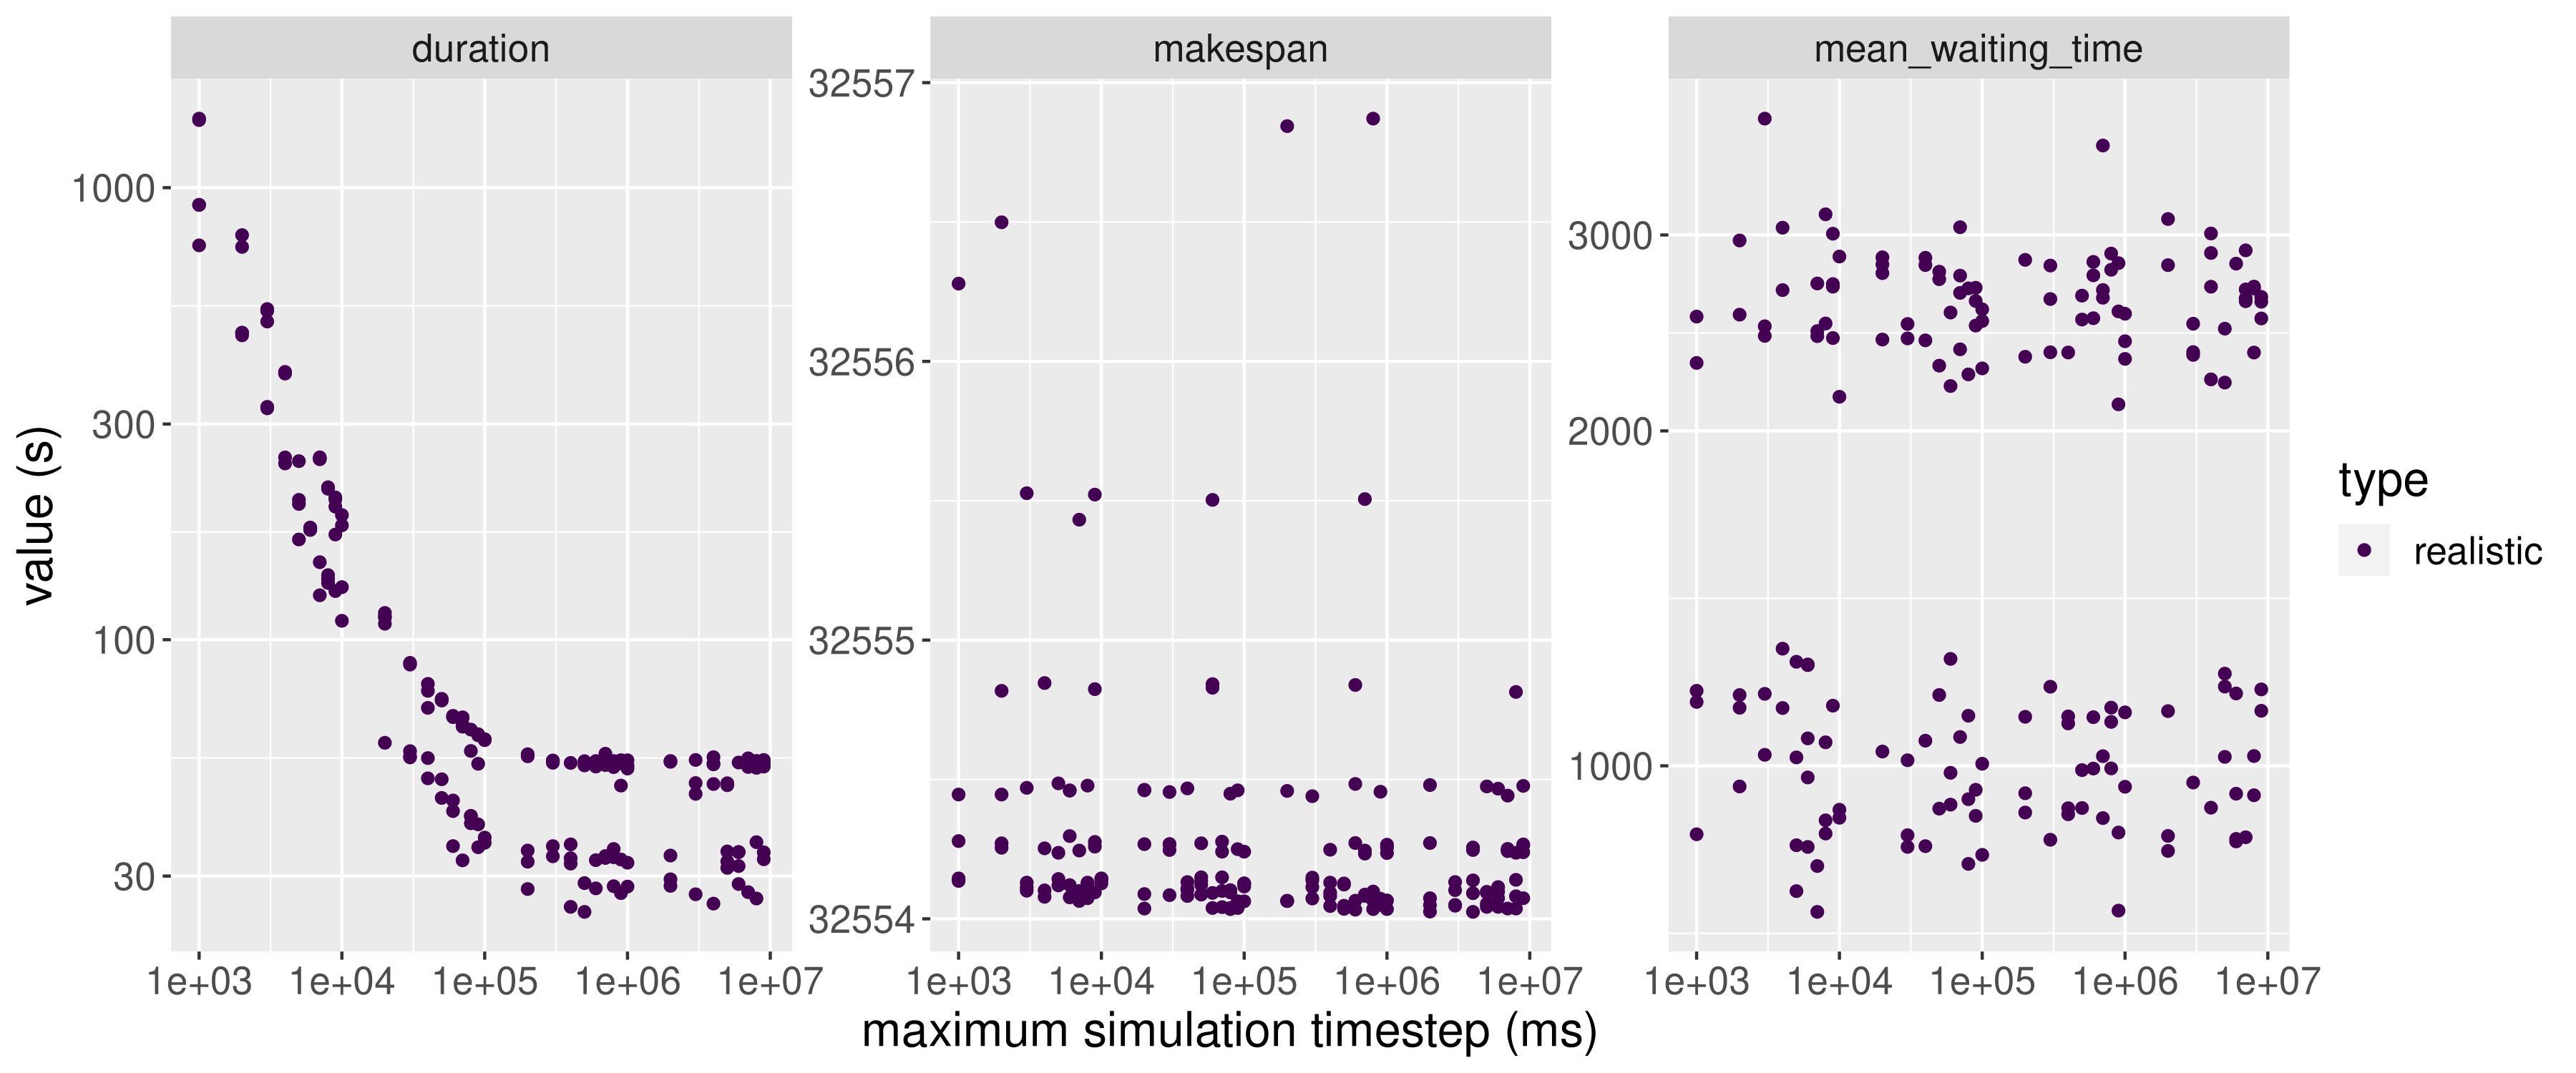
\includegraphics[width=\textwidth]{imgs/max-timestep_realistic.png}
		\caption{}
		\label{fig:timestep_real}
	\end{subfigure}

	\caption{Effect of the maximum simulation timestep on the simulation}
	\label{fig:timestep}
\end{figure}

As expected, the simulation time decreases drastically when the maximum
timestep increases. Still, this value reaches a minimum eventhough the maximum
timestep keeps increasing. This happens because Batsim events are only so far
appart in the simulation, and Batsim will always wake up before the maximum
timestep is reached.

Surprisingly, we observe that the increase in the maximum simulation timestep
has no noticeable effect on the other metrics for the burst and realistic
workloads. The makespan and mean waiting time flatten out regardless of the
increase in the timestep for the burst workload on figure
\ref{fig:timestep_burst_sp}. Regarding the realistic workload, we still observe
on figure \ref{fig:timestep_real} the different trajectories we noticed in the
last experiment, however the distribution does not change according to the
maximum timestep either.

\begin{figure}
	\begin{subfigure}{0.5\textwidth}
		\centering
		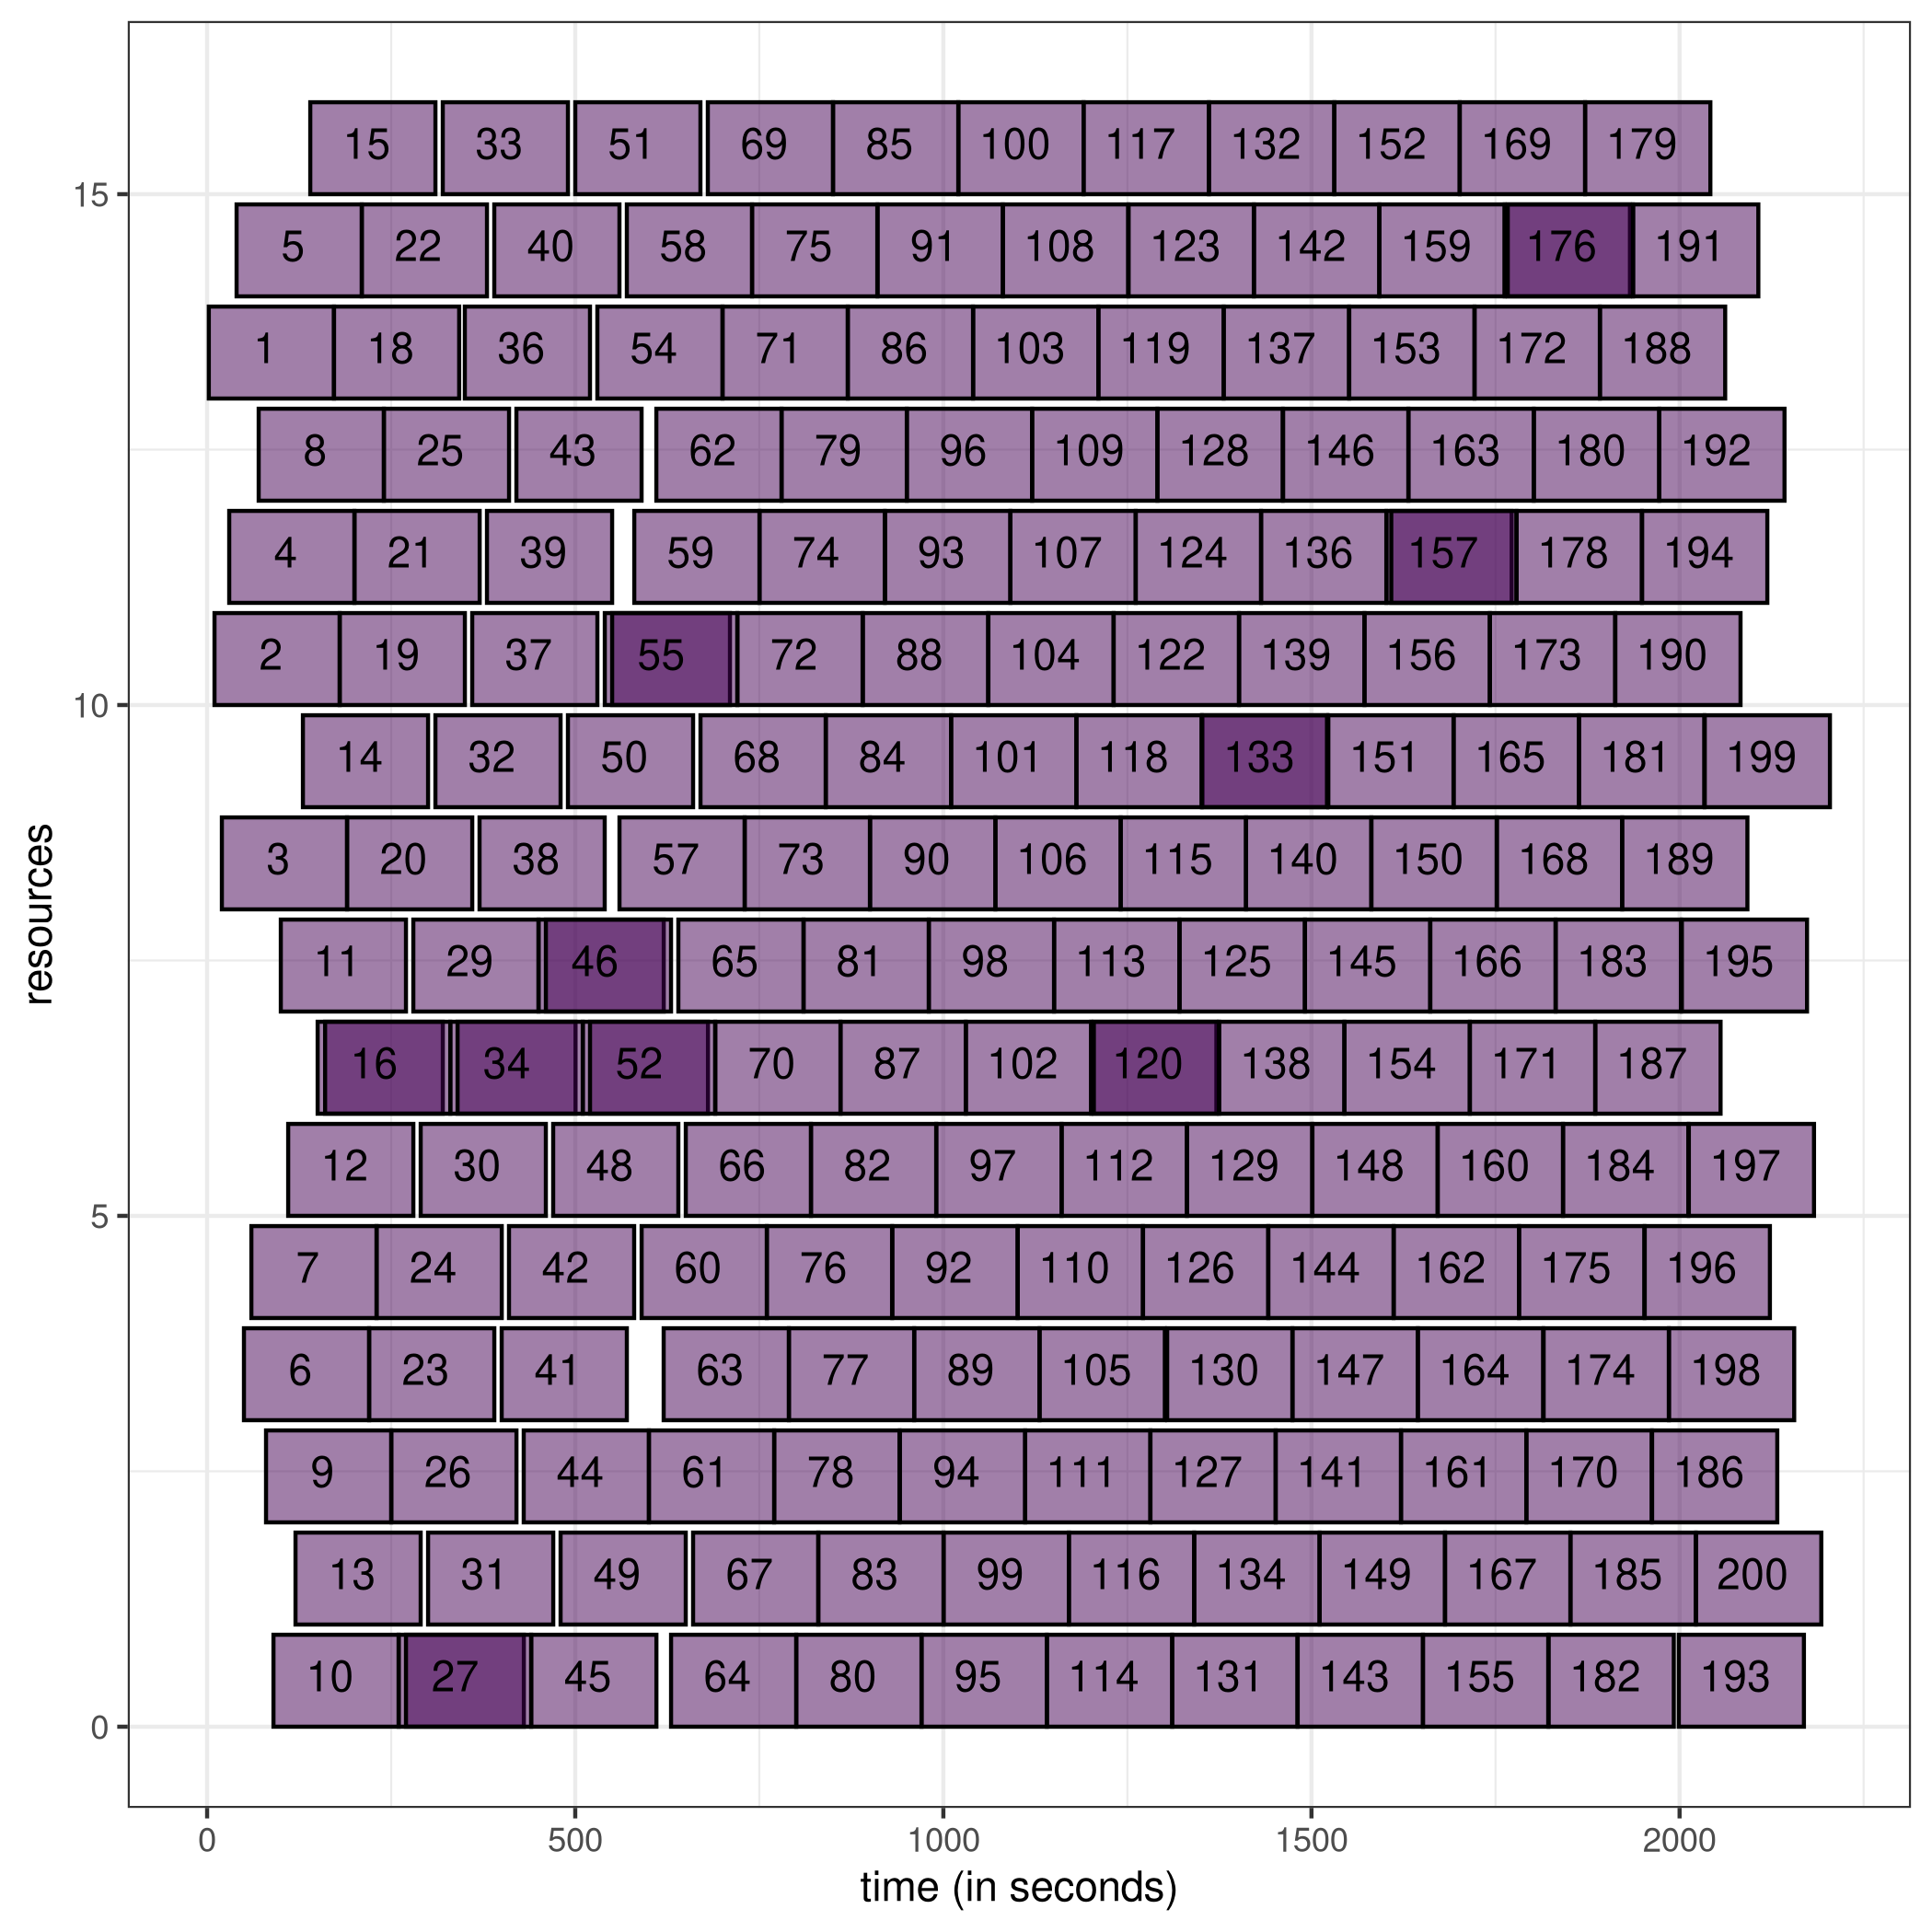
\includegraphics[width=\textwidth]{imgs/max-timestep_30ms_gantt.png}
		\caption{Maximum simulation timestep value: 30ms}
		\label{fig:timestep_5ms}
	\end{subfigure}
	\begin{subfigure}{0.5\textwidth}
		\centering
		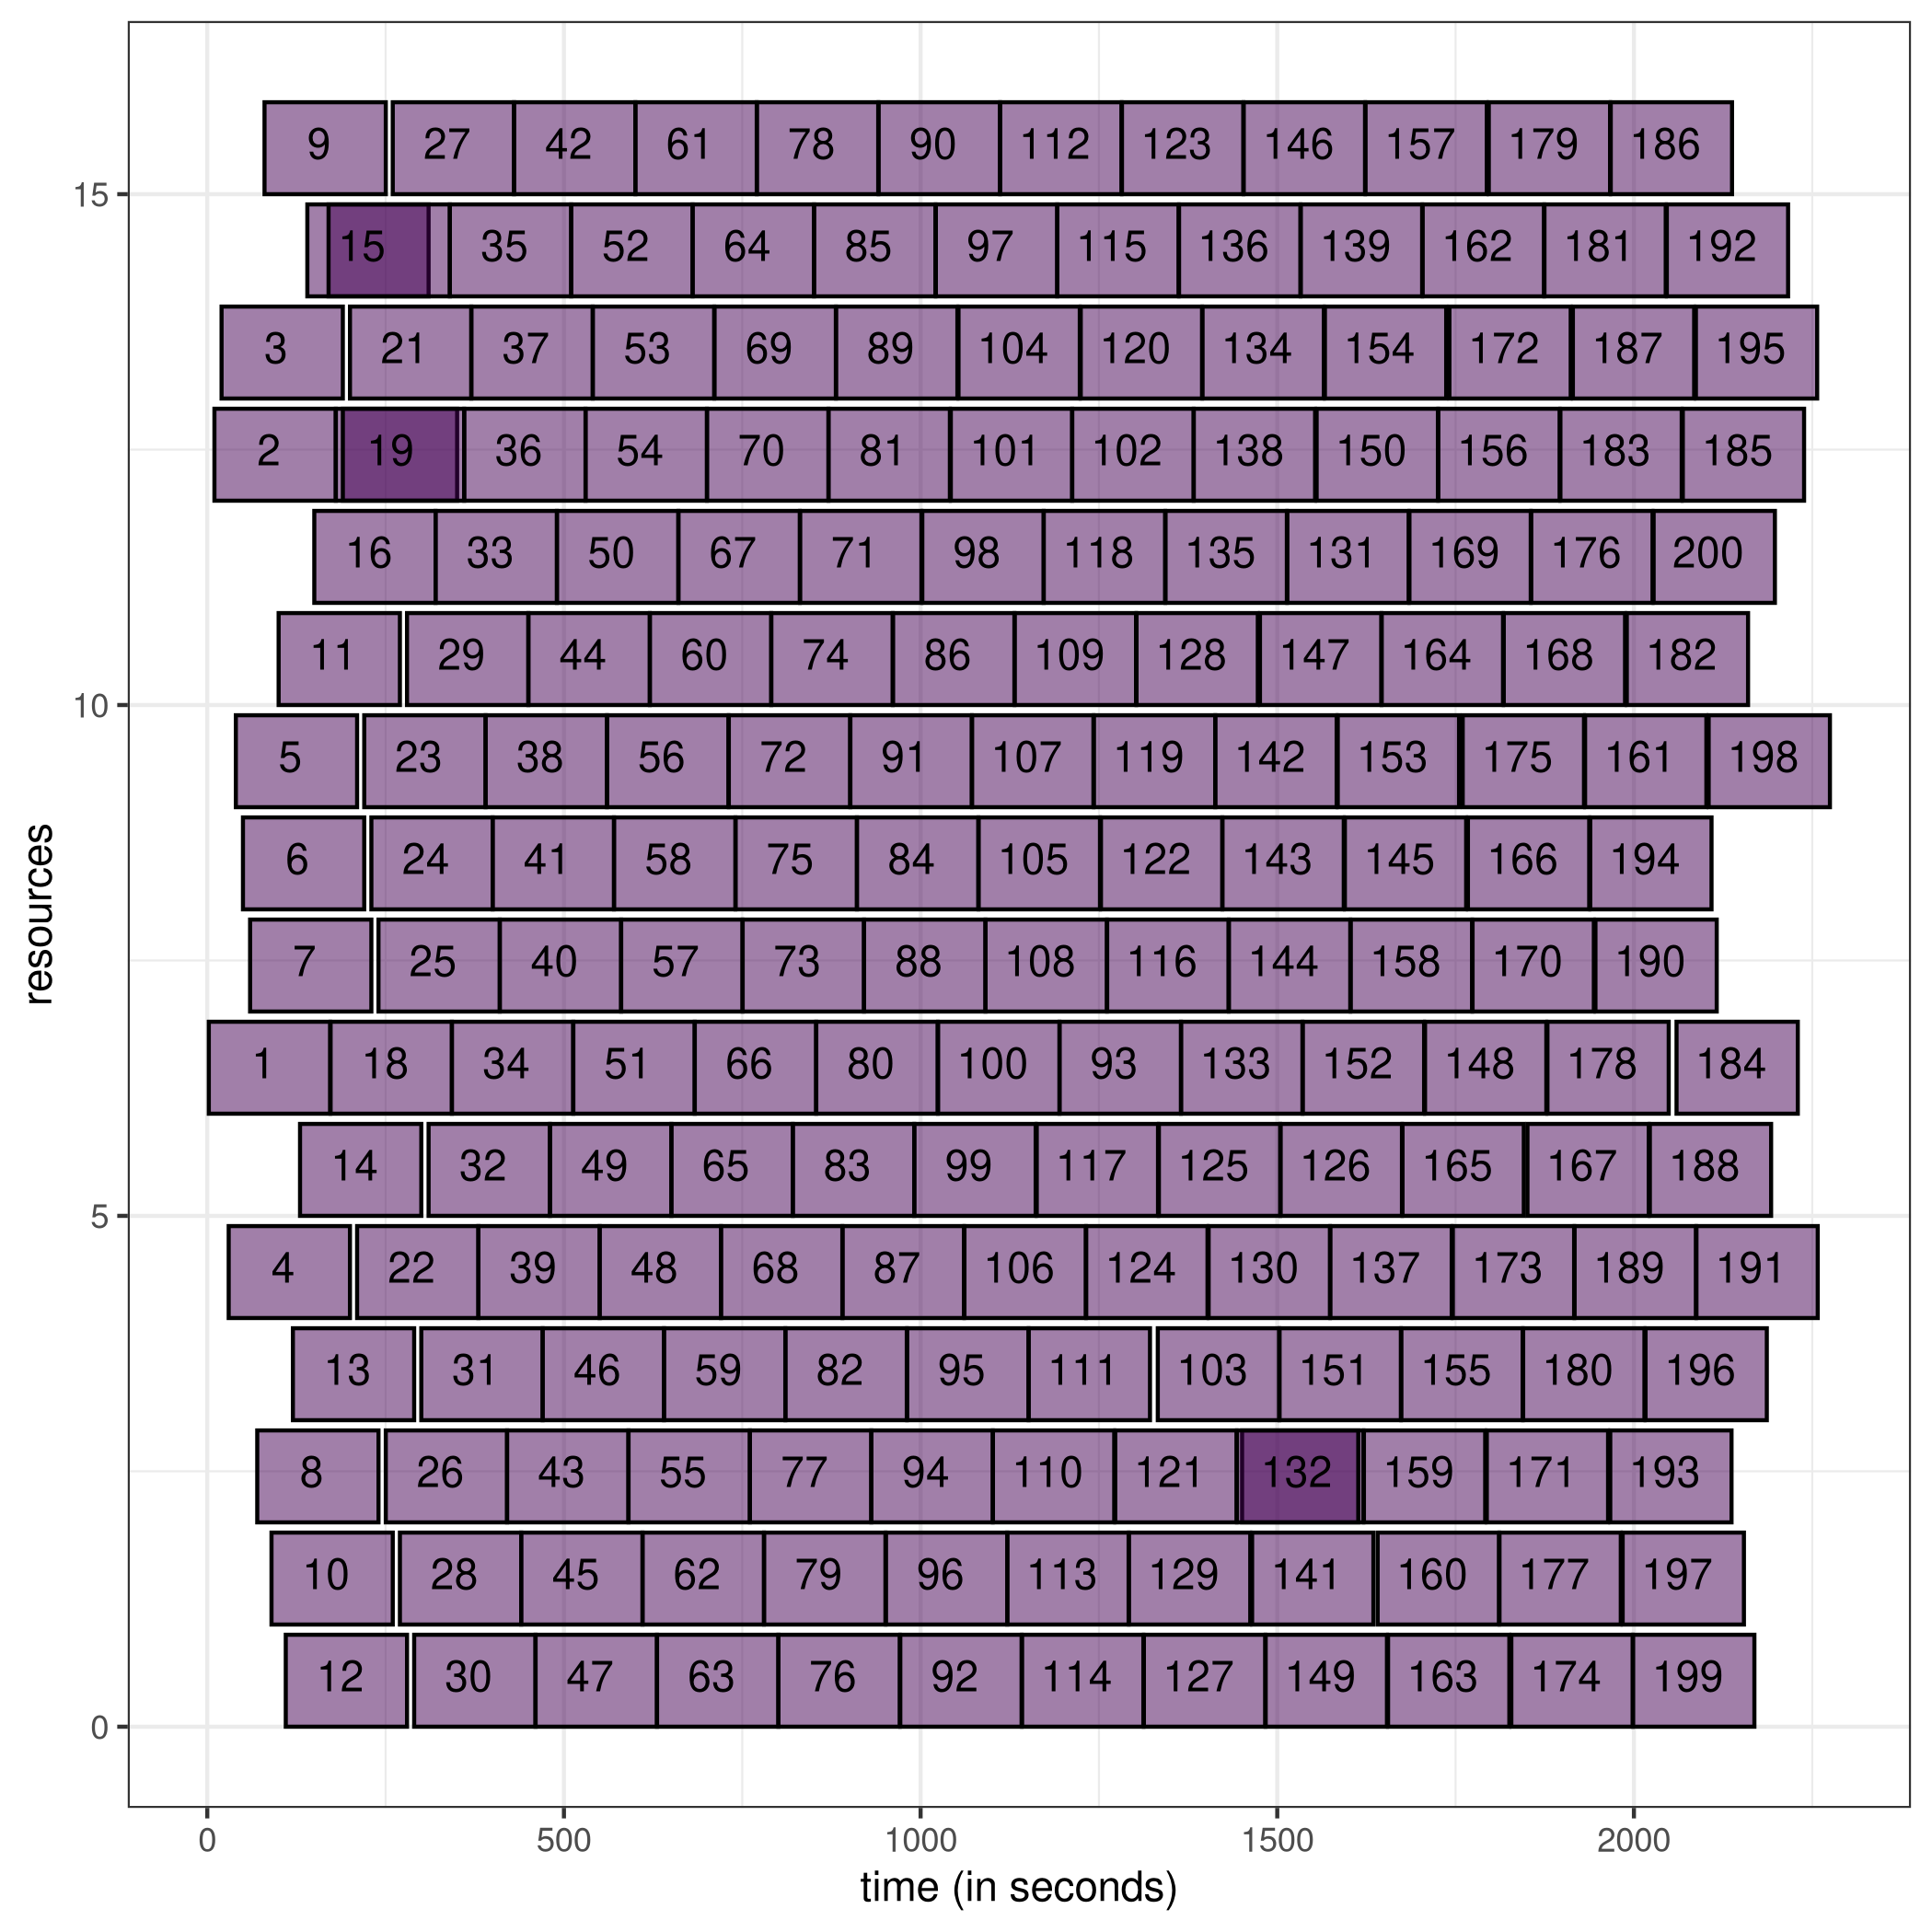
\includegraphics[width=\textwidth]{imgs/max-timestep_1000s_gantt.png}
		\caption{Maximum simulation timestep value: 1000s}
		\label{fig:timesteap_50ms}
	\end{subfigure}

	\caption{}
	\label{fig:timestep_overlap}
\end{figure}

The spaced workload however is impacted by the increase in the timestep.
Plotting a Gantt chart at different values of the simulation timestep allow us
to visualize why this happens, and it appears that lower values of the maximum
timestep induce more errors in the simulation. We believe that this is caused
by the drastic increase in the number of exchanges with the scheduler, which in
turn increases the likelihood of generating errors in the scheduler. We
conclude that having a low maximum timestep is never desirable, as it increases
both simulation time and scheduler errors. Furthermore, a timestep value as
high as 1000s in this case corresponds to no limits on Batsim jumps in time so
one could argue that this parameter can simply be discarded. While it is the
case here with these simple workloads and the absence of jobs preemption, it
might have an impact when the scheduler is susceptible to make scheduling
decisions on jobs that are already scheduled.

\section{Deviation of the simulation with reality}

Thanks to our emulated cluster we were able to run those same workloads on real
clusters that presented the same characteristics as the platforms we used to
run our simulations. The \textit{burst} and \textit{spaced} workloads were run
on 16 nodes each having one allocatable cpu, and the \textit{realistic}
workload was run on a single node composed of 6 allocatable cpus. The simulated
workloads were run with the following parameters : \texttt{min-delay=0ms},
\texttt{timeout-value=50ms}, \texttt{max-simulation-timestep=1000s}. Each
emulated workload was run 10 times (except for the realistic workload which was
only run once) and simulated workloads were run 20 times each. Here are the
deviations we observed between the simulation and the emulation.

As we saw earlier the scheduler makes errors in the simulations by allocating
pods on nodes that are already full. Also, the model is incomplete and the
simulator does not account for the time Kubernetes takes to pull the containers
from the Internet. For these reasons we except simulated makespan and mean
waiting time to be lower than the emulated ones.

\begin{table}
	\centering
	\begin{tabular}{|c|c|c|c|c|c|c|c|c|}
		\hline

		\multirow{3}{*}{} & \multicolumn{4}{c|}{\textbf{makespan}} & \multicolumn{4}{c|}{\textbf{mean waiting time}}\\

		\cline{2-9}

		& \multicolumn{2}{c|}{emulated} &
		\multicolumn{2}{c|}{simulated} & \multicolumn{2}{c|}{emulated}
		& \multicolumn{2}{c|}{simulated} \\

		\cline{2-9}

		& $\mu$ & $\sigma$ & $\mu$ & $\sigma$ & $\mu$ & $\sigma$ & $\mu$ & $\sigma$ \\
		
		\hline

		burst & 2467 & 28.3 & 2215 (-252) & 0.508 & 1077 & 10.6 & 970 (-107) & 12.6 \\
		spaced & 2468 & 5.14 & 2257 (-211) & 16.9 & 146 & 1.67 & 48.1 (-97.9) & 9.44 \\
		realistic & 32556 & - & 32555 (-1) & 1.30 & 2884 & - & 2020 (-864) & 950 \\
		\hline
	\end{tabular}
	\caption{Difference between emulated and simulated values. All values
	are in seconds. The difference with emulated results is indicating with
the simulated means.}
	\label{tab:deviation}
\end{table}

We observe a neat difference between simulated and emulated makespans for the
burst and spaced workloads as expected: the simulation does finish
earlier than the emulation. The mean waiting times of the burst workload seem
to follow this same principle as the simulated values are slightly lower than
emulated ones, although it doesn't seem to be the case for the spaced workload.
Indeed, the scheduler performed drastically better in the simulated scenario.
We don't know the cause of this. As for the realistic workload, the simulated
metrics correspond exactly to the ones measured in the emulated cluster. At
first glance, it seems that the waiting times do not correspond, however we
noticed during our experiments that the scheduler seemed to follow two
differents scenarios for this workload leading to two different values of the
mean waiting time.  This is especially obvious on figure
\ref{fig:timestep_real} where we notice two groups on the far right graph.
Considering this, we can make the assumption that the real waiting times values
either $\mu + \sigma$ or $\mu - \sigma$, that is to say, in this case, 2970 or
1070. We can then consider 2970 and 2884 to be part of the same group since
they are fairly close to each other and assume that the simulation was
accurate. Running more experiments with the emulated realistic workload would
give us better insights, unfortunately we did not have enough time on our
hands. In that regard, we would have benefited from a realistic workload
composed of more jobs and spanning over a shorter period of time. This is then
left for future work.

\section{Discussion and future work}

First, it is important to note some fundamental differences between Grid
Computing and Cluster Computing, differences because of which we had to put
aside large components of SimGrid models. Parallel computing relies on the
ability to schedule a task on multiple nodes.  The different processes
communicate with each others thanks to protocols such as the \textit{Message
Passing Interface (MPI)}. With Kubernetes however one cannot schedule one pod
on multiple nodes because it is not meant to run highly parallel tasks.
Furthermore, it would break the paradigm of encapsulation of containers within
nodes which is part of what make Kubernetes a powerful tool for cluster
administration.  Therefore, we are forced to ignore one of the major features
of SimGrid which is the simulation of parallel tasks and MPI applications
(SimGrid has an entire module for the simulation of MPI applications named SMPI
\cite{casanova:hal-01017319}).\\

Batkube, as a simulator, has limited features, however it is functional and the
fact that we were able to patch kube-batch in addition to the default scheduler
(it is mentioned in section \ref{sec:time-hijack}) proved that it is possible
to adapt any Kubernetes scheduler to Batsim, given further development on the
api. It supports delay jobs that can request resources such as cpu or memory.
In its current state the API supports the default Kubernetes scheduler, which
is  a very capable scheduler and is widely used in the industry. For now, it
can be improved in some ways.

The API of Batkube needs further development in order to correctly support
other Kubernetes schedulers. Partial or wrong implementations of the endpoints
lead to numerous bugs and misbehavior of the scheduler throughout the
development, and while the most critical issues have been resolved, some errors
remain like the over allocation of resources.

The obligatory synchronization of the time between the scheduler and Batsim
make this simulator not viable for large scale simulations. As we saw in the
experiments, a simple workload with 200 delay jobs of 170 seconds submitted
every 10 seconds already requires nearly two minutes of simulation. This is due
to the frequent exchanges between Batsim and Batkube over the json interface,
and the fact that we wait up to \textit{timeout value} every exchange. This is
why we did not conduct any scalability experiment. This kind of experiment
would require more time, but also more resources. Indeed, we observed that the
Kubernetes scheduler require more memory on long running experiments and
hindered our capacity of running long simulations. Also, not much work was put
into the scalability aspect of the simulator, because trying to improve its
performances before in its current state would be premature
optimisation\footnote{\url{http://wiki.c2.com/?RulesOfOptimization}}. This also is
left for future work.

Batkube simulation capabilities can be expanded on by implementing the rest of
Batsim own capabilities. A single pod cannot be scheduled on several nodes but
one node can still have a theoretically unlimited capacity in resources, and
pods inside one same node can communicate with each others and work together to
execute a parallel
task\footnote{\url{https://kubernetes.io/docs/concepts/workloads/controllers/job/}}.
With a bit of tweaking in the API one could model simple parallel tasks. Batsim
also supports energy models which could become a critical metric in the near
future, considering the climate urgency. Storage resoures can be added as well
for a more complete simulation of an online service with a database. Finally,
Batsim supports external events such as resource failures and other user
defined events.

With a deeper understanding of the Kubernetes api-server internals one could
support any other scheduler and compare them against each others. Also,
Kubernetes allowing the use of multiple schedulers, studies could be conducted
on their interaction with each other and how their combinations could improve
the general scheduling performances on various system topologies. Extensive
studies can be realized on schedulers competing with each others on the same
resources, justifying the need for a simulator. Also, since the api-server is
the central component of Kubernetes, any other tool of the k8s ecosystem could
be supported given a more complete API. During the development we already made
use of their command line interface, \texttt{kubectl}, to monitor the resources
and we could imagine plugging some monitoring tools to the simulator such as
\texttt{kubetop}. All this offer the perspective of a fully fledged Kubernetes
simulator based on the sound models of SimGrid.
